\documentclass[11pt,a4paper]{article}

% --- Packages ---
\usepackage[utf8]{inputenc}
\usepackage[margin=1in]{geometry}
\usepackage{amsmath,amssymb,amsthm,mathtools}
\usepackage{booktabs}
\usepackage{hyperref}
\usepackage[authoryear]{natbib}
\usepackage{tabularx}
\usepackage{float}
\usepackage{enumerate}

% --- Theorem Environments ---
\theoremstyle{definition}
\newtheorem{definition}{Definition}[section]

\theoremstyle{plain}
\newtheorem{theorem}{Theorem}[section]
\newtheorem{lemma}[theorem]{Lemma}
\newtheorem{proposition}[theorem]{Proposition}
\newtheorem{corollary}[theorem]{Corollary}

\theoremstyle{remark}
\newtheorem{remark}{Remark}[section]
\newtheorem{example}{Example}[section]

% --- Mathematical Operators ---
\DeclareMathOperator*{\argmax}{arg\,max}
\DeclareMathOperator*{\argmin}{arg\,min}
\newcommand{\E}{\mathbb{E}}
\renewcommand{\P}{\mathbb{P}}
\newcommand{\Q}{\mathbb{Q}}
\newcommand{\R}{\mathbb{R}}
\newcommand{\U}{\mathcal{U}}
\newcommand{\dee}{\mbox{d}}
\newcommand{\1}{\mathbf{1}}

\title{\textbf{Welfare Aggregation}}
\author{Isidor Hlebarov}
\date{12.10.2026}

\begin{document}

\maketitle

\section{General Idea}
\label{Sect:General_Idea}
To demonstrate how substituting the concave envelope changes (as in \citet{Dong2020}) the total fund welfare, the approximation error will be computed via the certainty equivalent (CE) loss. The goal is to measure the (percentage) difference between the CE coming from a Pareto-optimal allocation of risk under the true behavioral utility and the CE of the LEL-PEMC risk-sharing rule under the concave envelope to see whether the relaxation leads to economically significant reduction of welfare.

Because the KT utility function given in Section 4 of the thesis and defined on $[0, \infty)$ is strictly increasing, its inverse is well-defined and continuous:
\begin{equation*}
    u_{i,t}^{-1}(y) = \begin{cases} \text{ref}_{i,t} + y^{1/a} & \text{if } y \geq 0 \\ \text{ref}_{i,t} - \left( -\frac{y}{\eta} \right)^{1/b} & \text{if } -\eta (\text{ref}_{i,t})^b \leq y < 0 \end{cases}
\end{equation*}
For any candidate risk-sharing rule $W_{i,t+1}$, the certainty equivalent is:
\begin{equation*}
    \text{CE}_{i,t}(W_{i,t+1}) = u_{i,t}^{-1}(\E_t^{\P}(u_{i,t}(W_{i,t+1})))
\end{equation*}


\section{Market Dynamics}
The aggregate fund wealth at time $t+1$ is generated over a discrete period $[t,t+1]$ on a probability space $(\Omega, \mathcal{F}, \P)$. To assess how distributional shape influences welfare independently of the risk premium, all market settings are standardized to share the identical expected return $\E^\P(R) = 1+\mu$, except one of the scenarios where the equity premium is lowered, which will be described below. Rather than relying on continuous Monte Carlo draws that induce sample noise into the root-finding procedures, which are used frequently in computing the allocation rules, terminal returns are represented via a discrete scenario set of $M$ atoms (simulations), given by $\{(R^{(m)}, p^{(m)})\}_{m=1}^M$ with $\sum_{m=1}^M p^{(m)} = 1$. The log gross return $\log(R) = \log(W_{t+1}/W_t)$ is modeled as an $N$-component Gaussian mixture:
\begin{equation*}
    \log(R) \sim \sum_{j=1}^N w_j \mathcal{N}(\mu_j, \sigma^2_j)
\end{equation*}
with $w_j$ being the weight of the particular component of the mixture $j$. To ensure mean matching, the log returns are shifted by an affine constant:
\begin{equation*}
    c = \log(1 + \mu) - \log\left(\sum_{m=1}^M p^{(m)} \exp(\log(R^{(m)}))\right)
\end{equation*}
such that $\E^\P(R) = \sum_{m=1}^M p^{(m)} R^{(m)} = 1 + \mu$ holds identically. We utilize the following market scenarios (with the risk-free rate being 3\% in all scenarios):
\begin{enumerate}
    \item[A:] (GBM Base) A classic GBM with a single lognormal component $\sigma = 15\%$ and $\mu = 6\%$, reflecting the Black-Scholes dynamics from the original methodology proposal;
    \item[B:] (GBM Calm) Again a single lognormal component with low volatility $\sigma = 7\%$ and $\mu = 6\%$, where market shortfalls are rare and downside protection is inexpensive;
    \item[C:] (GBM Turbulent) A single lognormal component with severe volatility $\sigma = 30\%$ and $\mu = 6\%$, yielding frequent, deep deficits and expensive downside protection;
    \item[D:] (Fat Tails) A mixture of two normals - 90\% normal regime with same mean as above but $\sigma_1 = 10\%$ and 10\% volatile regime with $\mu_2 = -18\%$ and $\sigma_2 = 28\%$, preserving the overall volatility;
    \item[E:] (Crash Jump) A mixture of 96\% normal regime with same mean and volatility $\sigma_1 = 11\%$ and 4\% market crash regime with $\mu_2 = -42\%$ and $\sigma_2 = 9\%$ that frequently breaches downside floors;
    \item[F:] (Low Equity Premium) Identical to Scenario A volatility of 15\%, but with expected return of $\mu = 4\%$, which yields a 1\% risk premium above the 3\% risk-free rate, which penalizes the cost of downside guarantees.
\end{enumerate}


\section{Risk-Sharing Rules}
\label{Sect:Risk-Sharing_Rules}
To quantify the welfare losses coming from performing the LEL-CE allocation structure we consider the following eight allocation rules:
\begin{enumerate}
    \item \textbf{The Proportional Allocation}
    
    Similarly to what was done in Section 6 (Numerical Examples) of the thesis, we will consider the simple collective proportional sharing given by
    \begin{equation*}
        W_{i,t+1}^{\text{prop}} = \frac{W_{i,t}}{W_t} W_{t+1}
    \end{equation*}

    \item \textbf{The Proportional "Loser-Loses-All" Allocation} 
    
    By the Counter-monotonic Improvement Theorem the (possibly) randomized proportional "loser-loses-all" allocation, denoted by $W_{i,t+1}^{\text{prop LLA}}$, where the surplus is shared proportionally, following what was described in the Loss Aversion and Market Consistency document;
    \item \textbf{Optimal Capped "Loser-Loses-All" Allocation}
    
    Similar to the allocation above, we have a "loser-loses-all" allocation when again the "losers" are chosen at random, while the surplus is shared, following the Borch condition. The allocation is with a capped loss of $\delta = 0.20$ and denoted by $W_{i,t+1}^{\text{opt LLA (cap)}}$;

    \item \textbf{Optimal uncapped "Loser-Loses-All" Allocation}
    
    Like the allocation above but with the bound $\delta = 1$, leading to full exhaustion of the accumulated wealth when selected as a "loser". It is denoted by $W_{i,t+1}^{\text{opt LLA (free)}}$;
    \item \textbf{The LEL-CE Zero Loss Allocation}
    This mirrors the nominal (in the scenarios of the DNB) guarantee analyzed by \citet{KokkenNijmanWerker2024}, given by
    \begin{equation*}
        W_{i,t+1}^0 = \lim_{\epsilon \to 0} W_{i,t+1}^{\text{LEL-CE}},
    \end{equation*}
    where $W_{i,t+1}^{\text{LEL-CE}}$ is described in the next point;
    \item \textbf{The LEL-CE Allocation}
    
    This follows exactly the framework described in Section 4.6 of the thesis, that combines the ideas of \citet{NgNguyen2025} and \citet{Dong2020}, with the allocation denoted by $W_{i,t+1}^{\text{LEL-CE}}$. We take the bound $\epsilon = 0.005 \times W_{t}$;

    \item \textbf{The LEL-CE Randomized Allocation}
    
    The main issue with rules 2 and 3 is that they are only ex-post sharing rules, i.e., they do not determine and influence the aggregate wealth in the next period in any way. On the other hand, the LEL-CE enforces a trading strategy to achieve its bound. Therefore, a sensible approach is to randomize in a "loser-loses-all" fashion the LEL-CE aggregate to see the effects of randomization. It is denoted by $W_{i,t+1}^{\text{LEL-CE rand}}$ and is the randomization similarly to rules 3 and 4;

    \item \textbf{The Global Arrow-Debreu Optimum}
    
    This is the unconstrained global theoretical optimum under a complete-market loss aversion optimization. The idea is that now the investment strategy for the fund is also determined on the "loser-loses-all" basis, taking extreme bets, e.g., decreasing the probability of a loss, but increasing the magnitude of it if it occurs. It is denoted by $W_{i,t+1}^{\text{global AD}}$, and it serves as an upper bound for the problem.
\end{enumerate}
The last risk-sharing rule deserve more attention as it has not been treated before (for the other rules check the previous methodology and/or the MSc Thesis). Letting a fund aware of the "loser-loses-all" nature of optimal allocations choose not only the allocation structure but also the investment strategy leads to dropping the usual feasibility constraint and replacing it with an aggregate budget that the fund may trade. The social planner problem then is:
\begin{equation*}
    \max_{\{W_{i,t+1}\}} \sum_{i=1}^n \alpha_{i,t} \E_t^\P(\tilde{u}_{i,t}(W_{i,t+1})) \quad \text{s.t.} \quad \E_t^{\P}\left(\xi_{t+1} W_{i,t+1} \right) = W_{i,t},
\end{equation*}
where the last holds for all agents $i$. The problem is defined in terms of the concave envelope. The Lagrangian is given by
\begin{equation*}
    \mathcal{L} = \sum_{i=1}^n \alpha_{i,t} \E_t^\P(\tilde{u}_{i,t}(W_{i,t+1})) - \sum_{i=1}^n \lambda_{i,t} \left( \E_t^\P[\xi_{t+1} W_{i,t+1}] - W_{i,t} \right)
\end{equation*}
Solving the FOC leads to
\begin{equation*}
    \alpha_{i,t} \tilde{u}_{i,t}'(W_{i,t+1}) = \lambda_{i,t} \xi_{t+1}
\end{equation*}
The first-order derivative of the concave envelope is also piecewise and is
\begin{equation*}
    \tilde{u}_{i,t}'(x) = \begin{cases} a(x - \text{ref}_{i,t})^{a-1} & \text{if } x \ge z_i \\ c_{z_i} & \text{if } 0 \le x < z_i \end{cases}
\end{equation*}
with $z_i$ and $c_{z_i}$ as defined in the thesis. In prosperous states (low state price) the optimum lies in the concave branch, i.e., $W_{i,t+1} \geq z_i$, resulting in
\begin{equation*}
    W_{i,t+1}^* = \text{ref}_{i,t} + \left( \frac{\lambda_{i,t} \xi_{t+1}}{\alpha_{i,t} a} \right)^{\frac{1}{a-1}}
\end{equation*}
In downturn states (high state price), then the cost $\lambda_{i,t} \xi_{t+1} > \alpha_{i,t} c_{z_i}$ on $[0, z_i]$, the maximized at the boundary:
\begin{equation*}
    W_{i,t+1}^* = 0
\end{equation*}
Hence, the optimal allocation is:
\begin{equation*}
    W_{i,t+1}^* = \begin{cases} \text{ref}_{i,t} + \left( \frac{\lambda_{i,t} \xi_{t+1}}{\alpha_{i,t} a} \right)^{\frac{1}{a-1}} & \text{if } \xi_{t+1} < \frac{\alpha_{i,t} c_{z_i}}{\lambda_{i,t}} \\ 0 & \text{if } \xi_{t+1} \ge \frac{\alpha_{i,t} c_{z_i}}{\lambda_{i,t}} \end{cases}
\end{equation*}
Note that the Lagrange multiplier $\lambda_{i,t}$ is solved numerically as the unique root of:
\begin{equation*}
    \E_t^\P\left( \xi_{t+1} \left( \text{ref}_{i,t} + \left( \frac{\lambda_{i,t} \xi_{t+1}}{\alpha_{i,t} a} \right)^{\frac{1}{a-1}} \right) \1_{\left\{\xi_{t+1} < \frac{\alpha_{i,t} c_{z_i}}{\lambda_{i,t}}\right\}} \right) = W_{i,t}
\end{equation*}
Note that the optimal solution is defined for two specific regions of the concave envelope:
\begin{itemize}
    \item At $x=0$ we get that $\tilde{u}_{i,t}(0) = - \eta (\text{ref}_{i,t})^b = u_{i,t}(0)$;
    \item At all points $x \geq z_i$ we know that by construction $\tilde{u}_{i,t}(x) = u_{i,t}(x)$
\end{itemize}
Therefore, solving the social planner problem in the global Arrow-Debreu framework for the concave envelope is equivalent to solving the problem for the true loss aversion utility.


\section{Results}
\label{Sect:Results}
The results of the previously described simulations are given in Table \ref{tab:LEL_Results}, where we run 120 000 simulations with 10 identical agents. The loss aversion parameters are as in \citet{KahnemanTversky1992}, i.e., $a=b=0.88$ and $\eta = 2.25$.
\begin{table}[htbp]
  \centering
  \small
  \caption{Comparison of risk-sharing rules under different market settings}
  \label{tab:LEL_Results}
  \vspace{0.5em}
  % Custom centered column with wrapping:
  \newcolumntype{Y}{>{\centering\arraybackslash}X}
  \setlength{\tabcolsep}{3pt} % tighter horizontal padding between columns
  \begin{tabularx}{\textwidth}{l *{8}{Y}}
    \toprule
    \textbf{Market} & 
    \textbf{Prop} & 
    \textbf{Prop} \newline \textbf{LLA} & 
    \textbf{Opt LLA} \newline \textbf{(cap)} & 
    \textbf{Opt LLA} \newline \textbf{(free)} & 
    \textbf{LEL-CE} \newline \textbf{($\epsilon \to 0$)} & 
    \textbf{LEL-CE} & 
    \textbf{LEL-CE} \newline \textbf{rand} & 
    \textbf{Global} \newline \textbf{AD} \\
    \midrule
    A      & 0.98919 & 0.99137 & 0.99137 & 0.99722 & 0.99955 & 1.00092 & 1.00255 & 1.00488 \\
    B      & 1.00509 & 1.00940 & 1.00941 & 1.01459 & 1.00252 & 1.00879 & 1.02137 & 1.21038 \\
    C & 0.96030 & 0.96196 & 0.96196 & 0.97475 & 0.99981 & 1.00051 & 1.00051 & 1.00052 \\
    D     & 0.99491 & 0.99664 & 0.99664 & 1.00011 & 0.99989 & 1.00323 & 1.00449 & 1.01612 \\
    E    & 0.99423 & 0.99603 & 0.99603 & 0.99981 & 0.99987 & 1.00232 & 1.00359 & 1.01345 \\
    F   & 0.97819 & 0.98077 & 0.98077 & 0.98848 & 0.99987 & 1.00022 & 1.00022 & 1.00023 \\
    \bottomrule
  \end{tabularx}
\end{table}
The runtime of the full script is 669.0 seconds. Clearly the proportional rule is the biggest underperformer, given that it disregards completely the preferences of the agents. The proportional LLA rule improves on that, and sharing the surplus in a Borch-like fashion does not yield a meaningful improvement provided the loss limit of $\delta = 0.20$. Increasing the limit to $\delta = 1$ leads to improved welfare, due to the increased counter-monotonicity in the outcome. Then, applying the LEL-CE with $\epsilon \to 0$ is superior to the prior four allocation rules, but the lack of flexibility leads to welfare losses compared to the LEL-CE rule. Allowing for randomization logically leads to welfare improvement for the fund, but the difference is only largely noticeable for the calm market scenario. Finally, the global AD, which serves as the upper bound welfare, outperforms every other allocation. However, there is the caveat that it allows for unbounded leverage to achieve the "loser-loses-all" allocation, making it unrealistic for real-world pension funds. All-in-all, the LEL-CE looks like a promising alternative to randomized lotteries, preserving the "shared fate" principle. In Table \ref{tab:LEL_Results_Pct} we present the results in terms of percentage change relative to the LEL-CE allocation.
\begin{table}[htbp]
  \centering
  \small
  \caption{Percentage change of risk-sharing rules relative to the LEL-CE allocation (\%)}
  \label{tab:LEL_Results_Pct}
  \vspace{0.5em}
  % Custom centered column with wrapping:
  \newcolumntype{Y}{>{\centering\arraybackslash}X}
  \setlength{\tabcolsep}{3pt} % tighter horizontal padding between columns
  \begin{tabularx}{\textwidth}{l *{8}{Y}}
    \toprule
    \textbf{Market} & 
    \textbf{Prop} & 
    \textbf{Prop} \newline \textbf{LLA} & 
    \textbf{Opt LLA} \newline \textbf{(cap)} & 
    \textbf{Opt LLA} \newline \textbf{(free)} & 
    \textbf{LEL-CE} \newline \textbf{($\epsilon \to 0$)} & 
    \textbf{LEL-CE} \newline \textbf{(base)} & 
    \textbf{LEL-CE} \newline \textbf{rand} & 
    \textbf{Global} \newline \textbf{AD} \\
    \midrule
    A & $-1.17$ & $-0.95$ & $-0.95$ & $-0.37$ & $-0.14$ & $0.00$ & $0.16$  & $0.40$  \\
    B & $-0.37$ &  $0.06$ &  $0.06$ &  $0.57$ & $-0.62$ & $0.00$ & $1.25$  & $19.98$ \\
    C & $-4.02$ & $-3.85$ & $-3.85$ & $-2.57$ & $-0.07$ & $0.00$ & $0.00$  & $0.00$  \\
    D & $-0.83$ & $-0.66$ & $-0.66$ & $-0.31$ & $-0.33$ & $0.00$ & $0.13$  & $1.28$  \\
    E & $-0.81$ & $-0.63$ & $-0.63$ & $-0.25$ & $-0.24$ & $0.00$ & $0.13$  & $1.11$  \\
    F & $-2.20$ & $-1.94$ & $-1.94$ & $-1.17$ & $-0.04$ & $0.00$ & $0.00$  & $0.00$  \\
    \bottomrule
  \end{tabularx}
\end{table}
Finally, we also have the results in Table \ref{tab:welfare_diff_LEL} relative to the LEL-CE allocation as a percentage of the initial wealth.
\begin{table}[htbp]
  \centering
  \small
  \caption{Welfare difference relative to the LEL-CE allocation (\% of initial wealth $W_{i,t}$)}
  \label{tab:welfare_diff_LEL}
  \vspace{0.5em}
  % Custom centered column with wrapping:
  \newcolumntype{Y}{>{\centering\arraybackslash}X}
  \setlength{\tabcolsep}{3pt} % tighter horizontal padding between columns
  \begin{tabularx}{\textwidth}{l *{8}{Y}}
    \toprule
    \textbf{Market} & 
    \textbf{Prop} & 
    \textbf{Prop} \newline \textbf{LLA} & 
    \textbf{Opt LLA} \newline \textbf{(cap)} & 
    \textbf{Opt LLA} \newline \textbf{(free)} & 
    \textbf{LEL-CE} \newline \textbf{($\epsilon \to 0$)} & 
    \textbf{LEL-CE} \newline \textbf{(base)} & 
    \textbf{LEL-CE} \newline \textbf{rand} & 
    \textbf{Global} \newline \textbf{AD} \\
    \midrule
    A & $-1.21$ & $-0.98$ & $-0.98$ & $-0.38$ & $-0.14$ & $0.00$ & $0.17$  & $0.41$  \\
    B & $-0.38$ &  $0.06$ &  $0.06$ &  $0.60$ & $-0.65$ & $0.00$ & $1.30$  & $20.76$ \\
    C & $-4.14$ & $-3.97$ & $-3.97$ & $-2.65$ & $-0.07$ & $0.00$ & $0.00$  & $0.00$  \\
    D & $-0.86$ & $-0.68$ & $-0.68$ & $-0.32$ & $-0.34$ & $0.00$ & $0.13$  & $1.33$  \\
    E & $-0.83$ & $-0.65$ & $-0.65$ & $-0.26$ & $-0.25$ & $0.00$ & $0.13$  & $1.15$  \\
    F & $-2.27$ & $-2.00$ & $-2.00$ & $-1.21$ & $-0.04$ & $0.00$ & $0.00$  & $0.00$  \\
    \bottomrule
  \end{tabularx}
\end{table}


\section{Welfare Comparison under Heterogeneous Participants with Unique Social Planner Weights}
\label{Sect:Het_Participants_Unique_Weights}
The comparisons in Section \ref{Sect:Results} evaluate rules through certainty equivalent of a single representative agent, given the homogeneity of the participants in the pension scheme. Once members differ in their initial wealth or behavioral parameters, i.e., $(W_{i,t}, a_i, b_i, \eta_i)$, no representative agent is available. Comparing risk-sharing rules then becomes nontrivial. We need now an individual welfare measure, a way of weighting individuals and a scalar aggregate for the whole scheme. Throughout, we consider a pool of $n=5$ participants with $W_{i,t} \in \{0.5, 0.75, 1.0, 1.5, 2.25\}$ and KT parameters of $a=b=0.88$ and $\eta = 2.25$. The LEL-CE allocation with $\epsilon = 0.005 W_t$ is the baseline. 

Firstly, we formally define individual certainty equivalents and the percentage relative change relative to initial wealth for a specific risk-sharing rule.
\begin{definition}
    For allocation rule $k$ and participant $i$, the individual certainty equivalent and its percentage change relative to initial wealth are:
    \begin{equation}
        CE_{i,t}^k = u_{i,t}^{-1}\Big( \E_t^{\P}\big[u_{i,t}(W_{i,t+1}^k)\big] \Big), \qquad \%\Delta CE_{i,t}^k = 100 \times \frac{CE_{i,t}^k - CE_{i,t}^{\text{LEL-CE}}}{W_{i,t}},
    \end{equation}
    where $u_{i,t}$ is the true behavioral KT loss aversion utility function.
\end{definition}
If $CE_{i,t}^k \geq CE_{i,t}^{k'}$ for every $i$, we say that rule $k$ Pareto-dominates rule $k'$. The concave envelope $\tilde{u}_{i,t}$ is used to construct the LEL-CE rule, not to evaluate it. Its influence on how a rule is assessed is summarized by the relaxation effect
\begin{equation*}
    \Delta_i^{\text{CE}}(k) = u_{i,t}^{-1}\Big(\E_t^\P(\tilde{u}_{i,t}(W_{i,t+1}^k))\Big) - CE_{i,t}^k \geq 0,
\end{equation*}
the amount by which the concave envelope overstates the rule's certainty equivalent. It is zero whenever the allocation avoids the interval $(0, z_i)$, where the envelope and the true utility differ. The relaxation effect also has a direct economic interpretation. It equals the CE loss when members adhere to deterministic "shared fate" rather than exploiting the risk-seeking convexity of the loss domain. In Table \ref{tab:relaxation_effect} we showcase the relaxation effect for some of the rules in the heterogeneous pool.
\begin{table}[htbp]
  \centering
  \small
  \caption{Relaxation effect $\Delta_i^{\text{CE}}(k)$, in \% of $W_{i,t}$ (identical across members)}
  \label{tab:relaxation_effect}
  \vspace{0.5em}
  \begin{tabular*}{\textwidth}{@{\extracolsep{\fill}} l cccccc @{}}
    \toprule
    \textbf{Market} & \textbf{Prop} & \textbf{Prop LLA} & \textbf{LEL-CE ($\epsilon \to 0$)} & \textbf{LEL-CE} & \textbf{LEL-CE rand} & \textbf{Global AD} \\
    \midrule
    A & 0.8270 & 0.6030 & 0.1597 & 0.1682 & 0.0000 & 0.0000 \\
    B & 0.9785 & 0.5339 & 1.2529 & 1.2956 & 0.0000 & 0.0000 \\
    C & 1.4881 & 1.3171 & 0.0432 & 0.0000 & 0.0000 & 0.0000 \\
    D & 0.5360 & 0.3578 & 0.1467 & 0.1306 & 0.0000 & 0.0000 \\
    E & 0.5741 & 0.3891 & 0.1456 & 0.1295 & 0.0000 & 0.0000 \\
    F & 1.0598 & 0.7950 & 0.0264 & 0.0000 & 0.0000 & 0.0000 \\
    \bottomrule
  \end{tabular*}
\end{table}
Later we will show that for the LEL-CE rule, the relaxation effect equals the gain of its randomized version. For proportional sharing, it equals the gain of the uncapped optimal LLA rule over proportional sharing in Table \ref{tab:welfare_diff_LEL} of Section \ref{Sect:Results} of 0.83\% of $W_{i,t}$ in market $A$. The uncapped optimal LLA rule is precisely the concavification lottery of the proportional allocation. Essentially, the relaxation effect therefore measures the welfare that members give up when the fund does not randomize.

As shown by \citet{Pazderaetal2017} and \citet{NgNguyen2025}, the LEL-CE rule comes with a unique vector of market-consistent social planner Pareto weights $\alpha^*$. Following \citet{DavilaSchaab2025}, we hold these weights fixed across rules, so that differences in welfare are not driven by differences in weights. However, there are two important caveats. Firstly, the weights need a normalization. Replacing $u_{i,t}$ by $c_i u_{i,t}$ represents the same preferences with weight $\alpha_i/c_i$. Pareto weights acquire an interpersonal meaning only once utilities are normalized (see \citet{Harsanyi1955} and \citet{dAspremontGevers1977}). A possible normalization in the KT loss aversion case is at the reference outcome $\text{ref}_{i,t} = (1+r) W_{i,t}$. In our case this amounts to
\begin{equation}
    u^N_{i,t}(x)=W_{i,t}^{1-a}\,u_{i,t}(x)=W_{i,t}\,v(x/W_{i,t}),
\end{equation}
where $v$ is the KT utility per unit of contribution, i.e., 
\begin{equation}
    \label{eq:Loss_Averion_Per_Unit_Contribution}
    v(y) = \begin{cases} (y - (1+r))^a & \text{if } y \ge 1+r \\ -\eta ((1+r) - y)^a & \text{if } 0 \le y < 1+r \end{cases}
\end{equation}
for any $y = x/W_{i,t}$. Secondly, the market consistent weights are Negishi weights \citep{Negishi1960}. Each $\alpha_i^*$ is inversely proportional to member i's marginal utility of wealth when she invests her own wealth optimally. With common preferences, the LEL-CE allocation is homothetic and $\alpha_i^* \propto W_{i,t}^{1-a}$. In our pool, $\alpha^* = (0.1826, 0.1917, 0.1985, 0.2084, 0.2188)$, which is exactly uniform under the normalization. Moreover, every rule changes all participants' certainty equivalent by the same percentage, so every comparison is a Pareto comparison. Distributional trade-offs require heterogeneous preferences, which will be discussed in the example of Section \ref{Sect:Example}.

For fixed weights, we will define the notion of social certainty equivalent (SCE) using the Pareto-weighted social welfare maximizer:
\begin{equation}
    G_{\alpha}(c)=\max_{x\ge0,\ \sum_ix_i=c}\ \sum_{i=1}^n\alpha_i u_{i,t}(x_i).
\end{equation}
Then the SCE for rule $k$ is given by
\begin{equation}
    SCE^k_{\alpha}=G_{\alpha}^{-1}\Big(\sum_{i=1}^n\alpha_i\,\E^{\P}_t\big(u_{i,t}(W^k_{i,t+1})\big)\Big),
\end{equation}
which, for fixed $\alpha$, ranks rules exactly as the weighted sum of expected utilities does, while converting that sum into certain aggregate wealth. In the following proposition we establish the relation between the SCE and the individual CEs.
\begin{proposition}
\label{Prop:SCE_relation}
    If the function $G_{\alpha}: \mathbb{R}_+ \to \mathbb{R}$ is defined under the true loss aversion\footnote{In the sense of Section 4 in \citet{Hlebarov_2026_MSc_Thesis}.}, then for every rule and every weight vector
    \begin{equation*}
        \min_iCE^k_{i,t}\ \le\ SCE^k_\alpha\ \le\ \sum_iCE^k_{i,t}.
    \end{equation*}
\end{proposition}
The upper bound is reached when the CE vector is itself an efficient division (i.e., we have equalized weighted marginal utilities at the CEs for all agents) of $\sum_i CE_{i,t}^k$. This holds exactly under CARA \citep{Wilson1968} and identical CRRA preferences, and approximately for heterogeneous concave preferences. Note that under loss aversion the upper bound is not attained for which the $G$-function is responsible and not the specific rule. For tractably solving the model, $G$ is built from the concave envelopes. Hence, for a rule that gives every member the same relative certainty equivalent $y_k = CE_{i,t}^k/W_{i,t}$, the SCE has the closed from solution
\begin{equation}
    \label{eq:SCE_gap}
    SCE^k_{\alpha^*}=W_t\,\tilde v^{-1}\big(v(y_k)\big)\ \le\ W_t\,y_k=\sum_{i=1}^n CE^k_{i,t},
\end{equation}
where $\tilde{v}$ is the concave envelope of $v$. The inequality is strict whenever $y_k$ lies below the tangency point $z_i/W_{i,t}$. The Pareto-weighted maximizer $G$ values a sure aggregate as if it could be divided in a loser-loses-all fashion. Defining the efficiency gain of rule $k$ as
\begin{equation*}
    \mathcal{E}^k=\sum_{i=1}^n\big(CE^k_{i,t}-CE^{\text{LEL-CE}}_{i,t}\big),
\end{equation*}
we have that the SCE can be split into the efficiency gain and the SCE gap from \eqref{eq:SCE_gap}, in the spirit of \citet{DavilaSchaab2025}. Hence, in Table \ref{tab:welfare_relative_lel}, we exactly showcase this for some of the allocation rules we have been discussing and all market states.
\begin{table}[htbp]
  \centering
  \small
  \caption{Welfare relative to LEL-CE, in \% of $W_t$}
  \label{tab:welfare_relative_lel}
  \vspace{0.5em}
  \begin{tabular*}{\textwidth}{@{\extracolsep{\fill}} l rrrrrr @{}}
    \toprule
    \textbf{Market} & \textbf{Prop} & \textbf{Prop LLA} & \textbf{LEL-CE ($\epsilon \to 0$)} & \textbf{LEL-CE} & \textbf{LEL-CE rand} & \textbf{Global AD} \\
    \midrule
    \multicolumn{7}{@{}l}{\textit{\textbf{Panel A: Efficiency gain}}} \\
    \addlinespace[0.2em]
    A & $-1.2077$ & $-0.9837$ & $-0.1408$ & $0$ & $0.1682$ &  $0.4077$ \\
    B & $-0.3782$ &  $0.0663$ & $-0.6458$ & $0$ & $1.2956$ & $20.7640$ \\
    C & $-4.1417$ & $-3.9708$ & $-0.0714$ & $0$ & $0.0000$ &  $0.0009$ \\
    D & $-0.8559$ & $-0.6776$ & $-0.3430$ & $0$ & $0.1306$ &  $1.3287$ \\
    E & $-0.8343$ & $-0.6493$ & $-0.2541$ & $0$ & $0.1295$ &  $1.1450$ \\
    F & $-2.2696$ & $-2.0048$ & $-0.0365$ & $0$ & $0.0000$ &  $0.0000$ \\
    \midrule
    \multicolumn{7}{@{}l}{\textit{\textbf{Panel B: SCE gap}}} \\
    \addlinespace[0.2em]
    A & $-0.8089$ & $-0.6891$ & $-0.0760$ & $0$ & $0.0000$ & $0.0000$ \\
    B &  $0.0000$ &  $0.0000$ & $-0.0000$ & $0$ & $0.0000$ & $0.0000$ \\
    C & $-1.9387$ & $-1.8875$ & $-0.0400$ & $0$ & $0.0000$ & $0.0000$ \\
    D & $-0.4695$ & $-0.3452$ & $-0.0287$ & $0$ & $0.0000$ & $0.0000$ \\
    E & $-0.5143$ & $-0.3906$ & $-0.0319$ & $0$ & $0.0000$ & $0.0000$ \\
    F & $-1.3134$ & $-1.2067$ & $-0.0301$ & $0$ & $0.0000$ & $0.0001$ \\
    \bottomrule
  \end{tabular*}
\end{table}
From the discussion above, it is clear that summing up the values in the two panels above would lead to the raw SCE for each allocation rule $k$. Clearly the rules are ranked from left to right when it comes to efficiency in comparison to the LEL-CE rule. The SCE gap seems to be quite noticeable when it appears, resulting in a bit less than $2\%$ losses in some market states. We also showcase in Table \ref{tab:ce_distribution}, the summary statistics of the individual CE distribution across the agents.
\begin{table}[!htbp]
  \centering
  \small
  \caption{Individual Certainty Equivalent ($\text{CE}_i$) Distribution Across Agents}
  \label{tab:ce_distribution}
  \vspace{0.4em}
  \begin{tabular*}{\textwidth}{@{\extracolsep{\fill}} l rrrrrr @{}}
    \toprule
    Market Regime & Prop & Prop LLA & LEL-CE ($\epsilon \to 0$) & LEL-CE & LEL-CE rand & Global AD \\
    \midrule
    \multicolumn{7}{@{}l}{\textbf{Panel A: Minimum $\text{CE}_i$}} \\
    \addlinespace[0.2em]
    A     & $0.5094$ & $0.5106$ & $0.5148$ & $0.5155$ & $0.5163$ & $0.5175$ \\
    B      & $0.5176$ & $0.5198$ & $0.5163$ & $0.5195$ & $0.5260$ & $0.6233$ \\
    C  & $0.4946$ & $0.4954$ & $0.5149$ & $0.5153$ & $0.5153$ & $0.5153$ \\
    D     & $0.5124$ & $0.5133$ & $0.5149$ & $0.5167$ & $0.5173$ & $0.5233$ \\
    E    & $0.5120$ & $0.5130$ & $0.5149$ & $0.5162$ & $0.5168$ & $0.5219$ \\
    F   & $0.5038$ & $0.5051$ & $0.5149$ & $0.5151$ & $0.5151$ & $0.5151$ \\
    \midrule
    \multicolumn{7}{@{}l}{\textbf{Panel B: Maximum $\text{CE}_i$}} \\
    \addlinespace[0.2em]
    A       & $2.2925$ & $2.2975$ & $2.3165$ & $2.3196$ & $2.3234$ & $2.3288$ \\
    B     & $2.3293$ & $2.3393$ & $2.3232$ & $2.3378$ & $2.3670$ & $2.8051$ \\
    C  & $2.2255$ & $2.2293$ & $2.3171$ & $2.3187$ & $2.3187$ & $2.3187$ \\
    D     & $2.3057$ & $2.3097$ & $2.3172$ & $2.3250$ & $2.3279$ & $2.3548$ \\
    E     & $2.3041$ & $2.3083$ & $2.3172$ & $2.3229$ & $2.3258$ & $2.3487$ \\
    F    & $2.2670$ & $2.2729$ & $2.3172$ & $2.3180$ & $2.3180$ & $2.3180$ \\
    \midrule
    \multicolumn{7}{@{}l}{\textbf{Panel C: Interquartile Range (IQR $\text{CE}_i$)}} \\
    \addlinespace[0.2em]
    A       & $0.7642$ & $0.7658$ & $0.7722$ & $0.7732$ & $0.7745$ & $0.7763$ \\
    B      & $0.7764$ & $0.7798$ & $0.7744$ & $0.7793$ & $0.7890$ & $0.9350$ \\
    C  & $0.7418$ & $0.7431$ & $0.7724$ & $0.7729$ & $0.7729$ & $0.7729$ \\
    D      & $0.7686$ & $0.7699$ & $0.7724$ & $0.7750$ & $0.7760$ & $0.7849$ \\
    E     & $0.7680$ & $0.7694$ & $0.7724$ & $0.7743$ & $0.7753$ & $0.7829$ \\
    F    & $0.7557$ & $0.7576$ & $0.7724$ & $0.7727$ & $0.7727$ & $0.7727$ \\
    \midrule
    \multicolumn{7}{@{}l}{\textbf{Panel D: Mean Percentage Change in Certainty Equivalent ($\text{Mean }\%\Delta\text{CE}_i$)}} \\
    \addlinespace[0.2em]
    A      & $-1.2077$ & $-0.9837$ & $-0.1408$ & $0.0000$ & $0.1682$ &  $0.4077$ \\
    B       & $-0.3782$ &  $0.0663$ & $-0.6483$ & $0.0000$ & $1.2965$ & $20.7667$ \\
    C  & $-4.1417$ & $-3.9708$ & $-0.0714$ & $0.0000$ & $0.0000$ &  $0.0009$ \\
    D      & $-0.8559$ & $-0.6776$ & $-0.3430$ & $0.0000$ & $0.1306$ &  $1.3287$ \\
    E     & $-0.8343$ & $-0.6493$ & $-0.2541$ & $0.0000$ & $0.1295$ &  $1.1450$ \\
    F    & $-2.2696$ & $-2.0048$ & $-0.0365$ & $0.0000$ & $0.0000$ &  $0.0000$ \\
    \bottomrule
  \end{tabular*}
\end{table}
As we can see Panel D of Table \ref{tab:ce_distribution} coincides with Panel A from Table \ref{tab:welfare_relative_lel} coming from the way in which we have defined the efficiency gain.


\section{Welfare Comparison under Non-Unique Social Planner Weights}
\label{Sect:Non-Unique_Weights}
In Section \ref{Sect:Results} and \ref{Sect:Het_Participants_Unique_Weights}, the welfare comparisons are constructed based on a unique vector of Pareto weights. However, not imposing market consistency or working directly with non-convex behavioral preferences may lead to a set of possible social planner weights. Let $\mathcal{A}$ denote the set of admissible Pareto weights with
\begin{equation*}
    \mathcal{A} = \left\{ \alpha \in \mathbb{R}_{+}^n : \sum_{i=1}^n \alpha_i = 1 \right\}
\end{equation*}
Note that the definition above is more general, but, in principle, we can limit it to only the social planner weights that yield Pareto-efficient allocations.

When participants share identical behavioral parameters and wealth, i.e., they are homogeneous, any social planner function should treat equals equally ex-ante. Even if an ex-post allocation is supported by a set of possible weights $\mathcal{A}$, the set is invariant under permutations of the agents. Hence, the uniform Pareto weights (sometimes called uniform barycenter):
\begin{equation*}
    \alpha^* = \left( \frac{1}{n}, \dots, \frac{1}{n} \right)
\end{equation*}
collapses the set $\mathcal{A}$ to a unique social planner weight structure. The equal division allocation $x_i = c/n$ solves the maximum in the Pareto-weighted social welfare function $G_{\alpha, u}$, which now satisfies:
\begin{equation*}
    G_{\alpha}(c) = \max_{\sum_{i=1}^n x_i = c} \sum_{i=1}^n \alpha_i u(x_i) = \sum_{i=1}^n \frac{1}{n} u(c/n) = u(c/n)
\end{equation*}
Hence, the social certainty equivalent logically collapses to $SCE_{\alpha}^k = n CE_{i,t}^k$.

When agents are heterogeneous, no permutation symmetry exists. Consequently, evaluating rules under non-unique weights $\alpha \in \mathcal{A}$ requires systematic aggregation criteria that do not rely on an arbitrary single vector $\alpha$. To establish welfare comparisons robust to weight non-uniqueness over $\mathcal{A}$, we propose three complementary criteria:
\begin{enumerate}
    \item \textbf{Uniform Pareto Dominance across Admissible Weights}
    
    For any weight vector $\alpha \in \mathcal{A}$, the envelope SCE, denoted by $SCE_{\alpha, \tilde{u}}$, is computed via:
    \begin{equation*}
        SCE_{\alpha, \tilde{u}}^k = G_{\alpha, \tilde{u}}^{-1}\left( \sum_{i=1}^n \alpha_i \E_t^{\P}\big(\tilde{u}_{i,t}(W_{i,t+1}^k)\big) \right)
    \end{equation*}
    where $G_{\alpha, \tilde{u}}$ is the concave envelope version of the Pareto-weighted maximizer $G_{\alpha}$. Rule $k$ is said to uniformly dominate rule $k'$ on $\mathcal{A}$ if:
    \begin{equation*}
        SCE_{\alpha, \tilde{u}}^k \geq SCE_{\alpha, \tilde{u}}^{k'} \quad \forall \alpha \in \mathcal{A}
    \end{equation*}
    Uniform dominance ensures that rule $k$ is socially preferred regardless of the Pareto weights. This is a strong comparison criterion, hence we turn to a more robust specification;
    \item \textbf{Minimax (Worst-Case) Social Certainty Equivalent}
    
    When uniform dominance does not hold because rules exhibit distributional trade-offs across cohorts, the social planner may want to evaluate rule $k$ by its worst-case SCE over $\mathcal{A}$, following the idea robust individual choice under ambiguity framework of \citet{Gilboa_Schmeidler_1989_maxmin}, but adapted to our social planner choice, i.e.,
    \begin{equation}
        \underline{SCE}^{k}_{\mathcal{A}, \tilde{u}} = \inf_{\alpha \in \mathcal{A}} SCE_{\alpha, \tilde{u}}^k
    \end{equation}
    The corresponding robust percentage welfare difference relative to aggregate wealth is defined as:
    \begin{equation*}
        \% \Delta \underline{SCE}^{k}_{\mathcal{A}, \tilde{u}} = 100 \times \frac{\underline{SCE}^{k}_{\mathcal{A}, \tilde{u}} - \underline{SCE}^{\text{LEL-CE}}_{\mathcal{A}, \tilde{u}}}{W_t}
    \end{equation*}
    A positive value of $\% \Delta \underline{SCE}^{k}_{\mathcal{A}, \tilde{u}}$ indicates that even under the least favorable admissible welfare weighting, rule $k$ provides a higher guaranteed collective money-metric surplus than the baseline LEL-CE allocation;

    \item \textbf{Money-Metric Individual CE Aggregation}
    
    Because loss-averse utility functions $u_{i,t}$ are non-linear and reference-dependent, evaluating social welfare directly on expected utilities $\sum \alpha_i \E(u_i)$ conflates individual risk preferences with societal inequality aversion. Following \citet{Atkinson_1970} and \citet{Grantetal2010}, we decouple these dimensions by aggregating the vector of individual certainty equivalents directly. For a given inequality aversion parameter $\rho \geq 0$, the money-metric social planner aggregator is defined by:
    \begin{equation}
        W_{\text{CE}}^k(\alpha; \rho) = \begin{cases} \left( \sum_{i=1}^n \alpha_i (CE_{i,t}^k)^{1-\rho} \right)^{\frac{1}{1-\rho}} & \text{if } \rho \neq 1 \\ \exp\left( \sum_{i=1}^n \alpha_i \log(CE_{i,t}^k) \right) & \text{if } \rho = 1 \end{cases}
    \end{equation}
    When $\rho = 0$, $W_{\text{CE}}^k(\alpha; 0) = \sum_{i=1}^n \alpha_i CE_{i,t}^k$ represents the linear Pareto sum of individual certainty equivalents, measuring total risk-adjusted purchasing power. Evaluating $\inf_{\alpha \in \mathcal{A}} W_{\text{CE}}^k(\alpha; \rho)$ isolates the monetary welfare generated by the risk-sharing rule from shifts in interpersonal utility scaling, providing an operational scalar benchmark when $\alpha$ is set-valued.
\end{enumerate}
With heterogeneous participants the natural first step is to take $\mathcal{A} = \Delta_n$. This turns out to be uninformative as:
\begin{enumerate}
    \item The uniform dominance holds if and only if the rule Pareto-dominates in certainty equivalents;
    \item The maxmin SCE \citep{Gilboa_Schmeidler_1989_maxmin} equals $\min_i CE_{i,t}^k$, which is the CE of the worst-off member. With heterogeneous wealth this is simply the poorest member;
    \item The individual CE aggregation fails to work in its current shape as $\inf_\alpha W_{CE}(\alpha;\rho)=\min_iCE^k_{i,t}$ for every $\rho$, so the inequality-aversion parameter of the third criterion plays no role.
\end{enumerate}
The last two problems follow from Proposition \ref{Prop:SCE_relation}. Hence, non-uniqueness needs to be modelled by a restricted set of weights. We propose two such sets:
\begin{itemize}
    \item \textbf{Relaxed market consistency $\mathcal{A}_{\kappa}$}, which contains the weights for which the LEL-CE allocation, computed without its market-consistency step, transfers at most $\kappa W_{i,t}$ of market value to or from any member, with $\mathcal{A}_0 = \{\alpha^*\}$. Then, every admissible vector corresponds to a bounded deviation from market consistency;
    \item \textbf{Money-weight band $\mathcal{G}_{\kappa}$}, which contains the weights for which the social value of a euro to each member deviates by at most $100\kappa\%$ from that implied by $\alpha^*$ under the normalization discussed earlier in Section \ref{Sect:Het_Participants_Unique_Weights}. It is in the spirit of the social marginal welfare weights of \citet{SaezStantcheva2016}.
\end{itemize}
The two sets coincide only for moderately risk-averse members. A band value of transfers therefore translates into a range of weights that widens with risk aversion as the next Section \ref{Sect:Example} will show. Hence, now we can utilize the three comparison criteria from above but only apply them on $\mathcal{A}_{\kappa}$ or $\mathcal{G}_{\kappa}$ instead of the full simplex. The main change now is that the money-metric aggregation $W_{CE}(\alpha;\rho)$ is applied to CE returns $CE_{i,t}/W_{i,t}$ rather than CE levels, so that $\rho$ penalises unequal outcomes of the rule rather than unequal initial wealth \citep{Atkinson_1970}. We summarize each pairwise comparison by a robustness radius, which is the largest value of $\kappa$ for which rule $k$ dominates rule $k'$ on the admissible set. It has to be noted that $\mathcal{A}_{\kappa}$ is defined based on utility, while $\mathcal{G}_{\kappa}$ is money-metric. This brings the discussion on whether it is better to use utility levels or certainty equivalents. In the remaining analysis, especially in the example in Section \ref{Sect:Example} we will try to showcase why using utility levels might not be the best idea in some cases.


\section{Example: Two CRRA Members in a Lognormal Market}
\label{Sect:Example}
We consider a simple setting with two CRRA members in a lognormal market, which allows us to compute the two criteria in a closed form. The setting is given by:
\begin{itemize}
    \item Two members with equal contributions $W_{1,t} = W_{2,t} = 1$ and CRRA utility as defined in Section 2 of \citet{Hlebarov_2026_MSc_Thesis}. The utility is normalized as described in Section \ref{Sect:Het_Participants_Unique_Weights} with $\text{ref}_{i,t} = 1.03$. Participant 1 has risk aversion $\gamma_1 = 2$, while agent 2 has $\gamma_2 \geq 2$;
    \item We work in market A as a complete lognormal market, with a Sharpe ratio $\theta = 0.1914$;
    \item For simplicity a fund holds half its wealth in the risky asset and half in bonds (risk-free asset), so the aggregate payoff has a positive floor.
\end{itemize}
We will only compare the following three simple rules, in order to strip down the complexity of the risk-sharing rule and only focus on the machinery from Sections \ref{Sect:Het_Participants_Unique_Weights} and \ref{Sect:Non-Unique_Weights}:
\begin{enumerate}
    \item \textbf{P:} the proportional risk-sharing rule as discussed earlier;
    \item \textbf{B:} the Borch-efficient market-consistent sharing of the fund's payoff (i.e., the PEMC allocation from \citet{Hlebarov_2026_MSc_Thesis}\footnote{Apologies for citing the thesis so much.}), which redistributes a given aggregate like some of the ex post rules of Section \ref{Sect:Risk-Sharing_Rules};
    \item \textbf{M:} the complete-market PEMC rule, in which the fund is also allowed to choose the aggregate payoff. M can be thought of the CRRA counterpart of LEL-CE with a non-binding LEL constraint.
\end{enumerate}
Under M and due to market completeness, each member receives his Merton payoff, so $CE_i^M = \text{ref}_{i,t} e^{\theta^2/2\gamma_i}$. The market-consistent weights are $\alpha^*_i\propto e^{-\theta^2/(2\gamma_i)}$: unique, close to uniform and independent of the unit of account. Under the wealth scaling of CRRA utility, the same weights depend on the unit of account: with $\gamma_2=4$ they are $(0.48,\,0.52)$ when wealth is measured as $1$, and $(10^{-6},\,1)$ when the same wealth is measured as $1000$. Table \ref{tab:crra_findings} looks at various criteria for each of the three allocations in order to make a complete comparison. Each panel includes varying levels of risk aversion for the second member.
\begin{table}[!htbp]
  \centering
  \footnotesize
  \caption{Two CRRA members: utility aggregation (SCE) versus certainty-equivalent aggregation}
  \label{tab:crra_findings}
  \setlength{\tabcolsep}{2.5pt}
  \begin{tabular*}{\textwidth}{@{\extracolsep{\fill}} l rr rrrrr rrr @{}}
    \toprule
    & \multicolumn{2}{c}{Individual} & \multicolumn{5}{c}{Utility aggregation (SCE)} & \multicolumn{3}{c}{CE aggregation} \\
    \cmidrule(lr){2-3}\cmidrule(lr){4-8}\cmidrule(l){9-11}
    Rule & $CE_1$ & $CE_2$ & $\Delta SCE_{\alpha^*}$ & $\Delta SCE_{1/2}$ & $\min_{\mathcal A_{5\%}}\!\Delta SCE$ & $\hat\kappa_u$ & Gap & $\Delta\mathcal C_{\alpha^*}$ & $\hat\kappa_c$ & $\hat\kappa_g$ \\
         & (1) & (2) & (3) & (4) & (5) & (6) & (7) & (8) & (9) & (10) \\
    \midrule
    \multicolumn{11}{@{}l}{\textbf{Panel A:} $\gamma=(2,4)$;\ $\alpha^*=(0.4989,\,0.5011)$;\ $\mathcal A_{5\%}$: $\alpha_1\in[0.425,\,0.574]$} \\
    \addlinespace[0.2em]
    P & 1.03902 & 1.03320 & $-0.0993$ & $-0.0965$ & $-0.1123$ & ---    & 0.04 & $-0.0991$ & ---    & ---    \\
    B & 1.03943 & 1.03471 & $-0.0031$ & $-0.0031$ & $-0.0031$ & Pareto & 0.01 & $-0.0031$ & Pareto & Pareto \\
    M & 1.03948 & 1.03473 & $0$       & $0$       & $0$       & Pareto & 0.01 & $0$       & Pareto & Pareto \\
    \midrule
    \multicolumn{11}{@{}l}{\textbf{Panel B:} $\gamma=(2,16)$;\ $\alpha^*=(0.4980,\,0.5020)$;\ $\mathcal A_{5\%}$: $\alpha_1\in[0.291,\,0.713]$} \\
    \addlinespace[0.2em]
    P & 1.03902 & 1.00142 & $-1.8705$ & $-1.2959$ & $-3.7111$ & ---     & 35.97 & $-1.5167$ & ---     & ---     \\
    B & 1.03800 & 1.03100 & $-0.0825$ & $-0.0825$ & $-0.0816$ & 18.5\% & 0.01  & $-0.0822$ & 17.4\% & 94.1\% \\
    M & 1.03948 & 1.03118 & $0$       & $0$       & $0$       & Pareto  & 0.01  & $0$       & Pareto  & Pareto  \\
    \midrule
    \multicolumn{11}{@{}l}{\textbf{Panel C:} $\gamma_2\to\infty$;\ $\alpha^*\to(0.4977,\,0.5023)$} \\
    \addlinespace[0.2em]
    \multicolumn{11}{@{}l}{\quad\textit{$\gamma_2=256$;\ $\mathcal A_{5\%}$: $\alpha_1\in[3\cdot10^{-6},\,0.999998]$}} \\
    P & 1.03902 & 0.76314 & $-65.3207$ & $-64.0289$ & $-13.5616$ & ---     & 5195.10 & $-13.4303$ & ---    & ---     \\
    B & 1.03655 & 1.03005 & $-0.1476$  & $-0.1476$  & $-0.0018$  & 25.8\% & 0.00    & $-0.1469$  & 1.8\% & 99.1\% \\
    M & 1.03948 & 1.03007 & $0$        & $0$        & $0$        & Pareto  & 0.00    & $0$        & Pareto & Pareto  \\
    \addlinespace[0.2em]
    \multicolumn{11}{@{}l}{\quad\textit{$\gamma_2\to\infty$ (limit);\ $\mathcal A_{5\%}$: the open simplex}} \\
    P & 1.03902 & 0.51500 & $-77.7238$ & $-76.2238$ & $-25.7500$ & ---         & 5195.10 & $-25.8906$ & ---      & ---     \\
    B & 1.03642 & 1.03000 & $-0.1530$  & $-0.1530$  & $0.0000$   & $\to50\%$  & 0.00    & $-0.1523$  & $\to0$   & 99.9\% \\
    M & 1.03948 & 1.03000 & $0$        & $0$        & $0$        & Pareto      & 0.00    & $0$        & Pareto   & Pareto  \\
    \bottomrule
  \end{tabular*}
  \vspace{0.3em}

  \begin{minipage}{\textwidth}
  \footnotesize\textit{Notes:} Both members contribute $W_{i,t}=1$ ($W_t=2$); $\gamma_1=2$; market A; fund equity share $\pi_F=1/2$.
  Columns (3)--(5) and (8) are changes relative to M in \% of $W_t$.
  (3)~SCE at the market-consistent weights $\alpha^*$; since these weights are recomputed under any rescaling of utilities, the column does not depend on the normalisation.
  (4)~SCE with equal weights and the textbook scaling $u_i(x)=(x^{1-\gamma_i}-1)/(1-\gamma_i)$.
  (5)~Each rule evaluated at its own worst-case weights in $\mathcal A_{5\%}$, relative to the worst case of M.
  (6), (9)~Robustness radius of the rule over P on $\mathcal A_\kappa$, utility and CE version; (10)~on the money band $\mathcal G_\kappa$; ``Pareto'': the rule Pareto-dominates P.
  (7)~$\sum_iCE_i-SCE_{\alpha^*}$ in basis points of $W_t$.
  (8)~$\mathcal C_{\alpha^*}=n\sum_i\alpha^*_iCE_i$.
  Rows $\gamma_2\to\infty$ are analytic limits; there $\mathcal A_{5\%}$ is the open simplex and column (5) gives full-simplex values.
  \end{minipage}
\end{table}
Here is the explanation of the ten available columns:
\begin{enumerate}[(1)]
    \item $CE_1$: the certainty equivalent of agent 1;
    \item $CE_2$: the certainty equivalent of agent 2;
    \item $\Delta SCE_{\alpha^*}$, which uses the machinery from Section \ref{Sect:Het_Participants_Unique_Weights}, with the SCE being computed at the market-consistent weights;
    \item $\Delta SCE_{1/2}$, which uses the same machinery, but with equal weights, i.e., $\alpha_1 = \alpha_2 = 1/2$ as a robustness check;
    \item $\min_{\mathcal{A}_{5\%}} \Delta SCE$, which serves as the second criterion from Section \ref{Sect:Non-Unique_Weights} over the relaxed market consistency set;
    \item $\hat{\kappa}_u$, which is the Pareto-dominance criterion from Section \ref{Sect:Non-Unique_Weights}. Entries with "Pareto" mean the rule Pareto-dominates rule $P$;
    \item $\text{Gap} = \sum_i CE_i - SCE_{\alpha^*}$ as a basis point deviation from $W_t$;
    \item $\Delta \mathcal{C}_{\alpha^*}$, where $\mathcal{C}_{\alpha^*} = n \sum_i \alpha_i CE_i$, which is simply the CE counterpart of (3), with the weights being fixed;
    \item $\hat{\kappa}_c$ is the $\sum_i \alpha_i CE_i$, i.e., the second criterion from Section \ref{Sect:Non-Unique_Weights}, using the CE instead of the utility levels;
    \item $\hat{\kappa}_g$ is the same CE comparison on the money band $\mathcal{G}_\kappa$ as described in Section \ref{Sect:Non-Unique_Weights}.
\end{enumerate}
From Panel A, we clearly see that rule M is preferred over rule B, which is preferred over rule P in the Pareto sense. Every criterion gives the same ranking, where utility aggregation coincides with the CE one. Equal weights do not seem to matter a lot for welfare with every comparison being robust as all columns (6), (9) and (10) show Pareto-domination. Panel B becomes more interesting as the restricted sets become more information and the SCE starts to diverge from the sum of individual CEs. Relative to P, B raises $CE_2$ by 2.96\% of $W_{2,t}$ and lowers $CE_1$ by 0.10\%. The SCE becomes more sensitive to the choice of weights. B dominates P on $\mathcal{A}_{\kappa}$ up to $\kappa = 18.5\%$ in the utility version and $17.4\%$ in the CE version. B beats P on the money band up to $\kappa=94.1\%$, i.e. unless a euro to member 1 is valued more than 29 times a euro to member 2, coming from the definition of the money-band $\mathcal{G}_\kappa$. Clearly, the worst-case depends strongly on the weights as we can see in (5). From Panel C, however, we can see that utility aggregation fails to be informative. Here, the SCE rule collapses as P's SCE loss is -65.3, which is five times the CE-based loss of -13.4 for $\gamma_2 = 256$, where for $\gamma_2 \to \infty$ the values are -77.7 and -25.9 respectively. Clearly the three kappa columns diverge - $\hat{\kappa}_u$ stays bounded but rises from 18.5\% to 25.8\% and to 50\% in the limit. Hence, in the limit it measures only member 2's protection under P as $\pi_F = 50\%$. Moreover, $\hat{\kappa}_c$ collapses from 17.4\% to 1.8\% and to 0. At $\gamma_2 = 256$, a value of 1.8\% already admits weights of 108:1 in favor of member 1. In this case, only $\hat{\kappa}_g$ remains the robust measure.

Overall, it seems like that the social planner-based machinery from Sections \ref{Sect:Het_Participants_Unique_Weights} and \ref{Sect:Non-Unique_Weights} works well with concave utilities and moderate heterogeneity. However, utility-level aggregation fails when CEs lie below the reference points due to high risk aversion. Finally, relaxed market consistency using the set $\mathcal{A}_\kappa$ is a poor source of welfare weights whenever we have very risk-averse participants. This suggests the comparison in money rather than in utility units.


\section{Money-Metric Comparison of Risk-Sharing Rules}
\label{Sect:Money_Metric_Comparison}
The example of Section \ref{Sect:Example} showcased the problems with comparison welfare effects in utility units for heterogeneous agents. The SCE measure relies on normalization, includes the welfare loss from introducing the concave envelope, and it collapses when the CEs lie below the reference points. Money-metric comparison, by contrast, depends only on a member's ranking of lotteries in the KT case. It is unchanged by rescaling of the utility, needs no endogenous Pareto weights, and is continuous in the preference parameters. In the terminology of \citet{Fleurbaey2009} it is an equivalent income. We therefore propose to compare risk-sharing rules in money-metric terms, and to retain the analysis of Sections \ref{Sect:Het_Participants_Unique_Weights} and \ref{Sect:Non-Unique_Weights} as a robustness check.

\citet{FleurbaeyManiquet2011} argue that interpersonal comparisons should not compensate individuals for their preferences, where raw CEs fail in this requirement. Looking at the example in Section \ref{Sect:Example}, under the complete-market rule M, each member receives her own optimum. The more risk-averse member nonetheless has the lower CE return: in the example with $\gamma=(2,16)$, a maxmin criterion on CE returns would move 0.40\% of $W_{1,t}$ from member 1 to member 2, purely because member 2 is more risk-averse. We therefore measure each member by his equivalent contribution at market prices, the money-metric utility of \citet{McKenzie1957} and \citet{Samuelson1974} with state prices as reference prices:
\begin{equation}
    m_i^k = \min\left\{ \pi_t(X): \E_t^\P(u_{i,t}(X)) \geq \E_t^{\P}(u_{i,t}(W_{i,t+1}^k)) \right\}
\end{equation}
It is the contribution that, invested optimally by the member herself, leaves her as well off as rule $k$ does. Its properties are:
\begin{itemize}
    \item It represents the agent's preferences, as it depends only on her ranking of lotteries. Hence, Pareto comparisons in $m$ coincide with Pareto comparisons in expected utility;
    \item It does not compensate for specific preferences as we have that $m_i^k \leq \pi_t(W_{i,t+1}^k)$, with equality if and only if the member receives her own optimum. Participants with different risk attitudes who each receive their optimum all score $m_i/W_{i,t} = 1$ due to market consistency;
    \item It clearly separates redistribution from inefficiency without relying on endogenous Pareto weights. With value transfers $T_i^k = \pi_t(W_{i,t+1}^k) - W_{i,t}$ and deadweight loss $D_i^k = \pi_t(W_{i,t+1}^k) - m_i^k \geq 0$, i.e.,
    \begin{equation*}
        m^k_i-W_{i,t}=T^k_i-D^k_i,\qquad \sum_i\big(m^k_i-W_{i,t}\big)=-\sum_i D^k_i
    \end{equation*}
    The transfers cancel due to the feasibility constraint and market consistency, i.e., the fund's payoff being worth $W_t$. A rule that relaxes market consistency therefore show up through visible transfers, and not through unknown set of weights.
\end{itemize}
Going back to our CRRA example, we showcase equivalent contribution in the P and B rules for moderate and limit risk aversion in Table \ref{tab:equivalent_contribution_crra}.
\begin{table}[htbp]
  \centering
  \small
  \caption{Equivalent contribution $m_i / W_{i,t}$ in the CRRA example (rule M scores 1 for both members)}
  \label{tab:equivalent_contribution_crra}
  \vspace{0.5em}
  \begin{tabular*}{\textwidth}{@{\extracolsep{\fill}} l cccc @{}}
    \toprule
    & \textbf{P, $\gamma_2 = 16$} & \textbf{B, $\gamma_2 = 16$} & \textbf{P, $\gamma_2 = \infty$} & \textbf{B, $\gamma_2 = \infty$} \\
    \midrule
    Member 1 & 0.9996 & 0.9986 & 0.9996 & 0.9971 \\
    Member 2 & 0.9711 & 0.9998 & 0.5000 & 1.0000 \\
    \midrule
    $\Delta \Xi_0(k)$ (\% of $W_t$)      & $-1.4651$ & $-0.0800$ & $-25.0221$ & $-0.1472$ \\
    $\Delta \Xi_{0.5}(k)$ (\% of $W_t$)  & $-1.4703$ & $-0.0800$ & $-27.1558$ & $-0.1473$ \\
    $\Delta \Xi_1(k)$ (\% of $W_t$)      & $-1.4755$ & $-0.0800$ & $-29.3050$ & $-0.1473$ \\
    $\Delta \Xi_\infty(k)$ (\% of $W_t$) & $-2.8860$ & $-0.1424$ & $-50.0000$ & $-0.2944$ \\
    \bottomrule
  \end{tabular*}
\end{table}
Clearly, Pareto-efficient rule B does not diverge in this equivalent contribution even for extremely high risk aversion. For deterministic rules the efficiency gain of Table \ref{tab:welfare_relative_lel} remain the relevant numbers. The choice of individual measure matters once preferences differ. In this case distributional judgements enter through an explicit inequality-aversion parameter rather than through Pareto weights. The contribution-weighted \citet{Atkinson_1970} index of equivalent-contribution returns is
\begin{equation}
    \Xi_\rho(k)=\Big(\sum_i\frac{W_{i,t}}{W_t}\,\big(m^k_i/W_{i,t}\big)^{1-\rho}\Big)^{1/(1-\rho)},\qquad \rho \geq 0,
\end{equation}
where when $\rho = 0$ we have the efficiency measure from before in Section \ref{Sect:Het_Participants_Unique_Weights}, while $\rho \to \infty$ gives the maximin criterion favored by \citet{FleurbaeyManiquet2011}. In Table \ref{tab:equivalent_contribution_crra} the results for different values of the inequality aversion parameter $\rho$ relative to rule $M$ ($\Xi_\rho(M)=1$). We say that rule $k$ is preferred to $k'$ for every $\rho$ if it dominates in the generalized Lorenz sense of \citet{Shorrocks1983}. Hence, robustness over inequality aversion replaces the weights set of Section \ref{Sect:Non-Unique_Weights}. In the CRRA example, B dominates P in this sense both at $\gamma_2 = 16$ and $\gamma_2 \to \infty$, making it robust for every degree of inequality aversion, without any robustness radius and without any collapse in the limit.

Any criterion built on individual CE is ex ante as each member's lottery is evaluated from her own point of view, i.e., her own utility, before the outcome is known. Under loss aversion we have shown that by the Counter-monotonic Improvement Theorem \citep{Lauzier2024} this conflicts "shared fate". As each member in the loss aversion case will prefer a randomized loser-loses-all strategy of a rule over the rule itself, we should rank LEL-CE rand over LEL-CE and the optimal LLA rule above the proportional one as per Section \ref{Sect:Risk-Sharing_Rules}. This is the ex ante vs. ex post debate initially discussed by \citet{Diamond1967}'s critique of \citet{Harsanyi1955}. \citet{Fleurbaey2010} proposes to evaluate each realized state by the equally distributed equivalent (EDE) of the ex post distribution and take expectations. He shows that this is essentially the only approach compatible with statewise dominance, while full ex ante Pareto has to be given up. This idea essentially connects to the "shared fate" in that participants are not allowed to buy individual risk-seeking at the cost of ex post inequality among equals, i.e., among the other participants.

Hence, we will now look not at the overall distribution, but at the comparison between the ex ante and ex post analysis. Hence, we will look at the ex post SCE, which is the certain return received by every member in proportion to the individual contribution which is regarded as equally good as the rule. The idea is the unequal outcomes among identical members will be penalized with inequality aversion $\rho$, where the aggregate risk across states is valued with the preferences of each participant. Firstly, we fix the state $\omega$, which means that the market outcome and the outcome of the randomization device $U$ (uniform random variable for the lottery of loser-loses-all) are fixed. The equally distributed equivalent (EDE) of \citet{Atkinson_1970} is the common return that the fund regards as equivalent across the cross-section:
\begin{equation}
    e_\rho(\omega)=\Big(\sum_i \tfrac{W_{i,t}}{W_t} \left( \frac{W_{i,t+1}(\omega)}{W_{i,t}}\right)^{1-\rho}\Big)^{1/(1-\rho)}.
\end{equation}
For $\rho=0$ this is the contribution-weighted mean return, which is simply the aggregate return $W_{t+1}/W_t$. For $\rho>0$, $e_\rho(\omega)$ falls below the mean whenever returns differ, i.e., inequalities are punished, while for $\rho \to \infty$, it becomes the return of the worst-off member. Therefore, the rule now pays a risky return $e_\rho(\omega)$ to everyone, which is evaluated by the common loss aversion utility function per unit $v$ of contribution and reference point $(1+r)$, i.e.,
\begin{equation}
    SCE^{\text{ep}}_\rho=W_t\;v^{-1}\Big(\E^{\P}\big(v\big(e_\rho(\omega)\big)\big)\Big)
\end{equation}
with $v$ as in \eqref{eq:Loss_Averion_Per_Unit_Contribution}. The main idea is that the ex post SCE is in money and needs no Pareto weights, it does not depend on how $v$ is normalized and that lotteries are never rewarded. For $\rho=0$ it is worth exactly the underlying rule without randomization, while for $\rho>0$ it is strictly less, meaning that lotteries are punished. Again in our six market scenarios and six allocation rules that have been the focus from Section \ref{Sect:Het_Participants_Unique_Weights} onwards we construct Table \ref{tab:ex_post_vs_ex_ante} with three panels. In Panel A, we have the ex ante rule values, which are the same as the efficiency gains from Panel A of Table \ref{tab:welfare_relative_lel}. In Panel B, we look at the situation with $\rho=0$, while in Panel C, we consider $\rho=0.5$.
\begin{table}[!htbp]
  \centering
  \small
  \caption{Ex post vs ex ante comparison relative to LEL-CE, \% of $W_t$}
  \label{tab:ex_post_vs_ex_ante}
  \vspace{0.5em}
  \begin{tabular*}{\textwidth}{@{\extracolsep{\fill}} l rrrrrr @{}}
    \toprule
    \textbf{Market} & \textbf{Prop} & \textbf{Prop LLA} & \textbf{LEL-CE ($\epsilon \to 0$)} & \textbf{LEL-CE} & \textbf{LEL-CE rand} & \textbf{Global AD} \\
    \midrule
    \multicolumn{7}{@{}l}{\textit{\textbf{Panel A: Ex ante}}} \\
    \addlinespace[0.2em]
    A & $-1.2077$ & $-0.9837$ & $-0.1408$ & $0$ & $0.1682$ &  $0.4077$ \\
    B & $-0.3810$ &  $0.0636$ & $-0.6458$ & $0$ & $1.2956$ & $20.7640$ \\
    C & $-4.1417$ & $-3.9708$ & $-0.0714$ & $0$ & $0.0000$ &  $0.0009$ \\
    D & $-0.8558$ & $-0.6776$ & $-0.3429$ & $0$ & $0.1306$ &  $1.3287$ \\
    E & $-0.8343$ & $-0.6493$ & $-0.2541$ & $0$ & $0.1295$ &  $1.1450$ \\
    F & $-2.2688$ & $-2.0040$ & $-0.0357$ & $0$ & $0.0000$ &  $0.0008$ \\
    \midrule
    \multicolumn{7}{@{}l}{\textit{\textbf{Panel B: Ex post, $\rho = 0$}}} \\
    \addlinespace[0.2em]
    A & $-1.2077$ & $-1.2077$ & $-0.1408$ & $0$ & $0.0000$ &  $0.4077$ \\
    B & $-0.3810$ & $-0.3810$ & $-0.6458$ & $0$ & $0.0000$ & $20.7640$ \\
    C & $-4.1417$ & $-4.1417$ & $-0.0714$ & $0$ & $0.0000$ &  $0.0009$ \\
    D & $-0.8558$ & $-0.8558$ & $-0.3429$ & $0$ & $0.0000$ &  $1.3287$ \\
    E & $-0.8343$ & $-0.8343$ & $-0.2541$ & $0$ & $0.0000$ &  $1.1450$ \\
    F & $-2.2688$ & $-2.2688$ & $-0.0357$ & $0$ & $0.0000$ &  $0.0008$ \\
    \midrule
    \multicolumn{7}{@{}l}{\textit{\textbf{Panel C: Ex post, $\rho = 0.5$}}} \\
    \addlinespace[0.2em]
    A & $-1.2077$ & $-1.2696$ & $-0.1408$ & $0$ & $-0.2000$ &  $0.4077$ \\
    B & $-0.3810$ & $-0.4802$ & $-0.6458$ & $0$ & $-1.6191$ & $20.7640$ \\
    C & $-4.1417$ & $-4.1904$ & $-0.0714$ & $0$ &  $0.0000$ &  $0.0009$ \\
    D & $-0.8558$ & $-0.9027$ & $-0.3429$ & $0$ & $-0.2812$ &  $1.3287$ \\
    E & $-0.8343$ & $-0.8833$ & $-0.2541$ & $0$ & $-0.2473$ &  $1.1450$ \\
    F & $-2.2688$ & $-2.3421$ & $-0.0357$ & $0$ &  $0.0000$ &  $0.0008$ \\
    \bottomrule
  \end{tabular*}
\end{table}
Clearly, for the deterministic rules, i.e., the ones without randomization the values do not move across the three panels. The two lottery rules are punished in the ex post analysis and are therefore always weakly less preferred to the LEL-CE rule, which serves as the baseline. The ranking of the rules changes only for the lottery rules. Nevertheless, the zero loss LEL-CE rule remains the last in the calm state as strict guarantee is costly in calm markets. To be more specific, the difference between the ex ante values and the ex post one at $\rho=0$ can be considered as the price of "shared fate". It is the welfare that members forgo, by their own ex ante preferences, so that nobody inside the fund is singled out to bear the full loss. It essentially makes the concave-envelope relaxation to have the interpretation as the price of "shared fate". The Global AD rule does not change in the ex post analysis, because it is (optimally) an "all or nothing" rule across state of the world, but not across members. When it wipes out, it wipes out the wealth of all participants in the pension scheme. Hence, there are no inequalities within states of the world. This essentially means that the LEL-CE welfare loss comes from both the LEL constraint, i.e., the downside protection, and the lack of lottery, i.e., the deterministic implementation. The second loss is reconciled in the ex post analysis above. For the first consider the results in Table \ref{tab:LEL-CE_vs_Global_AD}, where the idea is to investigate further the behavior of the LEL-CE rand and the Global AD rule in comparison to the LEL-CE rule.
\begin{table}[htbp]
  \centering
  \small
  \caption{Comparison of LEL-CE and LEL-CE rand + Global AD}
  \label{tab:LEL-CE_vs_Global_AD}
  \vspace{0.5em}
  \begin{tabularx}{\textwidth}{@{} X l *{6}{r} @{}}
    \toprule
    \textbf{Benchmark} & \textbf{Criterion} & \textbf{A} & \textbf{B} & \textbf{C} & \textbf{D} & \textbf{E} & \textbf{F} \\
    \midrule
    (i) Price of "shared fate" (LEL-CE rand) & ex ante     &  0.17 &  1.30 & 0.00 &  0.13 &  0.13 & 0.00 \\
    & $\rho = 0$   &  0    &  0    & 0    &  0    &  0    & 0    \\
    & $\rho = 0.5$ & $-0.20$ & $-1.62$ & 0.00 & $-0.28$ & $-0.25$ & 0.00 \\
    \midrule
    (ii) Unconstrained investment and risk sharing (Global AD)      & every criterion &  0.41 & 20.76 & 0.00 &  1.33 &  1.15 & 0.00 \\
    \midrule
    \multicolumn{2}{@{}l}{Probability of fund wipe out: Global AD} & 1.9\% & 23.6\% & 0.3\% & 2.6\% & 3.1\% & 0.2\% \\
    \addlinespace[0.3em]
    \multicolumn{2}{@{}l}{Probability of fund wipe out: LEL-CE}    & 0.3\% &  0.2\% & 0.3\% & 0.2\% & 0.2\% & 0.2\% \\
    \bottomrule
  \end{tabularx}
\end{table}
Essentially, what we see in (i) is the price of "shared fate", which is at most 1.3\% ex ante, 0\% at $\rho$ and negative for $\rho>0$, where LEL-CE is strictly better, where we utilize the pool from Section \ref{Sect:Het_Participants_Unique_Weights}. Looking at (ii), which is computed in symmetric pool setting of Section \ref{Sect:Results}, we see that Global AD wins in every market state. Here, the ex ante vs ex post distinction does not matter, because we are looking at the price of downside protection. In markets C and F the LEL-CE and the Global AD rules are identical. The gains of Global AD in the other markets comes from severe risk-taking as we can see in the last two rows of the table. The 20.8\% welfare gains in the calm market, comes from an extreme leveraged position, which results in a 23.6\% fund wipe out probability, compared to the 0.2\% of the LEL-CE rule. In the base market LEL-CE only loses by 0.4\%, while in the severe downturn markets D and E the loss is 1.2-1.3\%. While the large gambles of the Global AD rule are acceptable for the loss aversion participants, they will not be such for a pension regulator. This goes to show that the LEL-CE creates a balance by paying a small price to restore "shared fate" and provide downside protection.


\section{Structural Overview and Comparison of Welfare Aggregation Criteria}
\label{Sect:Structural_Synthesis}
Sections \ref{Sect:Het_Participants_Unique_Weights}, \ref{Sect:Non-Unique_Weights}, \ref{Sect:Example} and \ref{Sect:Money_Metric_Comparison} develop two distinct paradigms for aggregating individual welfare across heterogeneous pension scheme participants when social planner weights are non-unique or market-consistency is relaxed. In Section \ref{Sect:Non-Unique_Weights}, non-uniqueness of the social planner weights $\alpha$ is handled by evaluating utility-based SCE via Uniform Dominance (Criterion 1), Minimax/Worst-Case SCE (Criterion 2), alongside a preliminary money-metric CES aggregator over raw certainty equivalents $W_{\text{CE}}^k(\alpha; \rho)$ (Criterion 3). Section \ref{Sect:Example} then demonstrates through the closed-form CRRA benchmark that utility-based aggregation and relaxed market consistency based sets $\mathcal{A}_{\kappa}$ suffer from severe structural distortions as risk aversion $\gamma$ increases. Finally, Section \ref{Sect:Money_Metric_Comparison} resolves these distortions by reformulating Criterion 3 around two money-metric ideas that require no Pareto weights. The first one is the Equivalent Contribution at Market Prices ($m_i^k$), aggregated across cohorts via the Atkinson index $\Xi_\rho(k)$ and the second one is the Ex-Post Social Certainty Equivalent $(SCE_{\rho}^{\text{ep}})$ which evaluates intra-state return dispersion via the Equally Distributed Equivalent $e_\rho(\omega)$. The idea of this section is to systematically compare Criterion 1 and Criterion 2 from Section \ref{Sect:Non-Unique_Weights} against the upgraded Criterion 3 from Section \ref{Sect:Money_Metric_Comparison} across four analytical dimensions. First, we will look at the behavior of each criterion when the social planner weights are unique ($\alpha = \alpha^*$). Then, we will analyze what happens to each criterion when market consistency is dropped ($\kappa > 0$), which will be followed by investigating whether the insights of Section \ref{Sect:Het_Participants_Unique_Weights} continue to hold. Finally, we will look at the sensitivity to variation in the degree of risk aversion, especially the case with extreme risk aversion ($\gamma_2 \to \infty$) as in Section \ref{Sect:Example}. It has to be noted that the analysis is organized along two structural comparisons - individual welfare metric (utilitarian vs. money-metric) and interpersonal aggregation device (weight set vs. inequality aversion parameter). We also look at the orthogonal ex-ante vs. ex-post solidarity axis.

\subsection{The Three Aggregation Criteria in Unified Form}
To place the three criteria on a common footing for any candidate risk-sharing rule $k$ and baseline rule (such as the LEL-CE in Sections \ref{Sect:Het_Participants_Unique_Weights} and \ref{Sect:Non-Unique_Weights} and $M$ in Section \ref{Sect:Example}), we summarize their operational definitions in their final form:
\begin{enumerate}
    \item \textbf{Criterion 1: Uniform SCE Dominance (Section \ref{Sect:Non-Unique_Weights})}
    
    Given an admissible set of Pareto weights $\mathcal{A}_\kappa$ induced by relaxing market consistency up to a maximum value transfer of $\kappa W_{i,t}$, rule $k$ uniformly dominates rule $k'$ if and only if:
    \begin{equation}
        SCE_{\alpha}^k \ge SCE_{\alpha}^{k'} \quad \forall \alpha \in \mathcal{A}_\kappa,
    \end{equation}
    where $SCE_{\alpha}^k = G_{\alpha}^{-1}\left(\sum_{i=1}^n \alpha_i \E_t^{\P}[u_{i,t}(W_{i,t+1}^k)]\right)$. Pairwise comparisons are summarized by the utility robustness radius $\hat{\kappa}_u = \sup\{\kappa \ge 0 : SCE_{\alpha}^k \ge SCE_{\alpha}^{k'} \, \forall \alpha \in \mathcal{A}_\kappa\}$, which measures the largest departure from market consistency under which all admissible planners agree on the ranking;
    \item \textbf{Criterion 2: Maxmin/Worst-Case SCE (Section \ref{Sect:Non-Unique_Weights})}
    
    When distributional trade-offs across participants prevents uniform dominance on $\mathcal{A}_\kappa$ ($\kappa > \hat{\kappa}_u$), a social planner evaluates rule $k$ by its worst-case collective value over the admissible weight set:
    \begin{equation}
        \underline{SCE}_{\mathcal{A}_\kappa}^k = \inf_{\alpha \in \mathcal{A}_\kappa} SCE_{\alpha}^k
    \end{equation}
    and ranks rules via the worst-case relative difference $\%\Delta \underline{SCE}_{\mathcal{A}_\kappa}^k = 100 \times (\underline{SCE}_{\mathcal{A}_\kappa}^k - \underline{SCE}_{\mathcal{A}_\kappa}^b)/W_t$;
    \item \textbf{Criterion 3: Money-Metric Aggregation (Section \ref{Sect:Money_Metric_Comparison})}
    
    Rather than aggregating raw certainty equivalents $CE_{i,t}^k / W_{i,t}$ over an unknown weight set $\alpha \in \mathcal{A}$ as in the preliminary specification of Section 6, the upgraded Criterion 3 of Section \ref{Sect:Money_Metric_Comparison} decouples efficiency, preference heterogeneity, and ex-post solidarity through two weight-free money-metric aggregators:
    \begin{itemize}
        \item \textbf{Criterion 3a (Ex-Ante Equivalent-Contribution Index:)}
        
        Each member's welfare is measured by her equivalent contribution at reference state prices, $m_i^k = \min\{\pi_t(X) : \E_t^{\P}[u_{i,t}(X)] \geq \E_t^{\P}[u_{i,t}(W_{i,t+1}^k)]\}$, and aggregated across the scheme via the contribution-weighted Atkinson index:
        \begin{equation}
            \Xi_\rho(k) = \left( \sum_{i=1}^n \frac{W_{i,t}}{W_t} \left( \frac{m_i^k}{W_{i,t}} \right)^{1-\rho} \right)^{\frac{1}{1-\rho}}, \quad \rho \ge 0
        \end{equation}
        Rule $k$ robustly dominates rule $k'$ across all degrees of societal inequality aversion $\rho \ge 0$ if and only if the vector of equivalent-contribution returns $(m_i^k / W_{i,t})_{i=1}^n$ Generalized Lorenz dominates $(m_i^{k'} / W_{i,t})_{i=1}^n$.

        \item \textbf{Criterion 3b (Ex-Post Solidarity Index):}
        
        To evaluate rules that introduce ex-post dispersion among identical members via randomization (Prop LLA, Opt LLA, LEL-CE rand), cross-sectional returns within each realized state $\omega$ are first compressed via the Equally Distributed Equivalent
        \begin{equation*}
            e_\rho(\omega) = \left(\sum_{i=1}^n \frac{W_{i,t}}{W_t} (W_{i,t+1}^k(\omega)/W_{i,t})^{1-\rho}\right)^{1/(1-\rho)}
        \end{equation*}
        and then evaluated under the per-unit behavioral utility $v$:
        \begin{equation}
            SCE_\rho^{\text{ep}} = W_t \, v^{-1}\left( \E_t^{P}\big[ v(e_\rho(\omega)) \big] \right)
        \end{equation}
    \end{itemize}
\end{enumerate}

\subsection{Unique Social Planner Weights}
When market consistency is strictly enforced ($\kappa=0$), the admissible set of social planner weights collapses to the unique $\alpha^*$ as established in Section \ref{Sect:Het_Participants_Unique_Weights}, i.e., $\mathcal{A}_0 = \{\alpha^*\}$. This has the following implications for the criteria:
\begin{itemize}
    \item Criteria 1 and 2 collapse to $SCE_{\alpha^*}^k$, because of the admissible set being a singleton. Hence, quantification over $\mathcal{A}_0$ (Criterion 1) and infimum evaluation over $\mathcal{A}_0$ (Criterion 2) become identical. Both criteria essentially become the Social Certainty Equivalent $SCE_{\alpha^*}^k$ analyzed in Section \ref{Sect:Het_Participants_Unique_Weights};
    \item Criteria 3a with $\rho=0$ now isolates the pure allocation efficiency. By the decomposition of Section \ref{Sect:Money_Metric_Comparison}, $m_i^k - W_{i,t} = T_i^k - D_i^k$, where $T_i^k = \pi_t(W_{i,t+1}^k) - W_{i,t}$ is the market-value transfer and $D_i^k = \pi_t(W_{i,t+1}^k) - m_i^k \ge 0$ is the individual deadweight loss. Because market-consistent rules satisfy $T_i^k = 0$ for all $i$ (and feasibility leads to $\sum_{i=1}^n T_i^k = 0$ identically), evaluating Criterion 3a at $\rho = 0$ yields:
    \begin{equation*}
        W_t \big( \Xi_0(k) - 1 \big) = \sum_{i=1}^n (m_i^k - W_{i,t}) = -\sum_{i=1}^n D_i^k \le 0
    \end{equation*}
    Thus, at unique weights $\alpha^*$ and $\rho=0$, Criterion 3a measures the exact Kaldor-Hicks efficiency gain (as in \citet{DavilaSchaab2025}) that Criteria 1 and 2 try to approximate in utility units;
    \item In the heterogeneous-wealth KT pool of Section \ref{Sect:Het_Participants_Unique_Weights}, where preferences are homothetic, the difference between Criteria 1-2 ($SCE_{\alpha^*}^k$), and Criterion 3 ($\sum_i CE_{i,t}^k$) at unique $\alpha^*$ is precisely the SCE gap reported in Panel B of Table \ref{tab:welfare_relative_lel}. This gap arises because the Pareto-weighted maximizer $G_{\alpha^*}$ values sure aggregate wealth as if it could be split in a "loser-loses-all" fashion whenever $CE_{i,t}^k < z_i$. Simultaneously, comparing Criterion 3a (ex-ante efficiency) with Criterion 3b ($SCE_0^{\text{ep}}$ at $\rho = 0$) in Table \ref{tab:ex_post_vs_ex_ante} isolates the concave envelope relaxation effect $\Delta_i^{\text{CE}}(k)$ of Table \ref{tab:relaxation_effect} as the exact price of "shared fate", i.e., the ex-ante certainty equivalent members forgo to avoid being singled out by an ex-post lottery.
\end{itemize}

\subsection{Relaxed Market Consistency}
When market consistency is dropped, a risk-sharing rule may induce cross-subsidies across the participants ($T_i^k \neq 0$), which also means that the Pareto weights $\alpha$ are no longer unique. Now we will discuss how this non-unique set of weights propagates in our criteria:
\begin{itemize}
    \item As shown in Section \ref{Sect:Non-Unique_Weights} (Proposition \ref{Prop:SCE_relation}), if market consistency is dropped without restriction, we get that $\mathcal{A} = \Delta_n$. This makes Criteria 1 and 2 uninformative, because Criterion 1 reduces to unweighted Pareto dominance for each agent, i.e., $CE_{i,t}^k \geq CE_{i,t}^{k'}$ for all $i$, while Criterion 2 collapses to the poorest member's certainty equivalent $\min_i CE_{i,t}^k$. That is why, in order to avoid full simplex degeneracy, we restrict $\alpha$ to the relaxed market-consistency neighborhood $\mathcal{A}_{\kappa}$, as proposed in Section \ref{Sect:Non-Unique_Weights}. However, this only treats departures from market consistency indirectly through an unobservable set of utility weights;
    \item However, in Criterion 3a of Section \ref{Sect:Money_Metric_Comparison}, the requirement for a set of endogenous Pareto weights disappears completely. Because $m_i^k - W_{i,t} = T_i^k - D_i^k$, any departure from market consistency is recorded directly as an observable financial transfer $T_i^k = \pi_t(W_{i,t+1}^k) - W_{i,t}$, while normative trade-offs between gainers and losers are evaluated transparently across the scalar inequality-aversion curve $\rho \mapsto \Xi_\rho(k)$ using fixed contribution weights $W_{i,t}/W_t$. Note that at $\rho \to \infty$, $\Xi_\infty(k) = \min_i (m_i^k / W_{i,t})$ is the money-metric counterpart of Criterion 2 on the full simplex ($\min_i CE_{i,t}^k$), while requiring $\Xi_\rho(k) \geq \Xi_\rho(k')$ for all $\rho \geq 0$ (Generalized Lorenz dominance) is strictly weaker than unweighted Pareto dominance ($m_i^k \geq m_i^{k'} \ \forall i$) but stronger than comparing means alone ($\rho = 0$).
\end{itemize}

\subsection{Relation to Insights from Section \ref{Sect:Het_Participants_Unique_Weights}}
Whether the three criteria reproduce the policy rankings of Section \ref{Sect:Het_Participants_Unique_Weights} depends on whether heterogeneity is confined to initial wealth or extends to preference parameters and ex-post randomization:
\begin{itemize}
    \item \textbf{Deterministic Rules under Wealth Heterogeneity Alone (Participant Pool of Section \ref{Sect:Het_Participants_Unique_Weights})}
    
    When participants differ in initial contributions $W_{i,t} \in \{0.5, 0.75, 1.0, 1.5, 2.25\}$ but share identical homothetic KT preferences ($a = b = 0.88, \eta = 2.25$), every rule $k$ changes every participant's relative certainty equivalent $CE_{i,t}^k / W_{i,t}$ and equivalent contribution $m_i^k / W_{i,t}$ by the exact same proportion. Hence, every comparison we made in Section \ref{Sect:Het_Participants_Unique_Weights} is a Pareto comparison, in the sense that we look at the efficiency of each risk-sharing allocation. Dropping market consistency or changing the aggregation criterion leaves the insights from Section \ref{Sect:Het_Participants_Unique_Weights} unchanged. Criteria 1, 2, 3a and 3b all rank deterministic rules in the exact order of Table \ref{tab:welfare_relative_lel}, i.e., Prop $<$ LEL-CE ($\epsilon \to 0$) $<$ LEL-CE $<$ Global AD in five of the six market regimes, with LEL-CE ($\epsilon \to 0$) ranking last in the calm market B. It has to be noted that the invariance of the rankings holds by construction as we have identical homothetic KT preferences with the rules being homothetic as well;
    \item \textbf{Randomized Rules (Prop LLA and LEL-CE rand)}
    
    Here, Criteria 1, 2, and 3a diverge from Criterion 3b. Because Criteria 1, 2, and 3a evaluate each participant's lottery ex ante, the Counter-monotonic Improvement Theorem \citep{Lauzier2024} dictates that they strictly prefer randomized "loser-loses-all" rules (LEL-CE rand $\succ$ LEL-CE and Prop LLA $\succ$ Prop), matching Panel A of Table \ref{tab:welfare_relative_lel} and Panel A of Table \ref{tab:ex_post_vs_ex_ante}. Criterion 3b ($SCE_\rho^{\text{ep}}$), however, evaluates the realized cross-sectional distribution ex post within each state $\omega$. As shown in Panels B and C of Table \ref{tab:ex_post_vs_ex_ante}, at $\rho = 0$ the lottery gain vanishes (LEL-CE rand ties with LEL-CE at $0.0000\%$), and for any $\rho > 0$ (e.g., $\rho = 0.5$), LEL-CE rand is strictly inferior to LEL-CE ($-0.2000\%$ in Market A and $-1.6191\%$ in Market B). Thus, Criterion 3b is the unique criterion that formally rationalizes the preference for deterministic "shared fate" over randomized lotteries;

    \item \textbf{Preference Heterogeneity (Section \ref{Sect:Example} CRRA Pool)}
    
    Once participants differ in risk aversion ($\gamma_1 \neq \gamma_2$), risk-sharing rules generate cross-sectional trade-offs (e.g., rule $B$ versus rule $P$ in Table \ref{tab:crra_findings}), and the three criteria no longer yield identical insights.
\end{itemize}

\subsection{Sensitivity to Risk-Aversion Heterogeneity}
The two-agent CRRA example in Section \ref{Sect:Example} ($\gamma_1 = 2$ and $\gamma_2 \in \{4, 16, 256, \infty\}$) provides an exact stress test of how the three criteria respond as preference heterogeneity widens. Criterion 3b is excluded in this discussion because a common per-unit utility $v$ is undefined when $\gamma_1 \neq \gamma_2$.
\begin{itemize}
    \item \textbf{Regime 1: Mild Risk-Aversion Dispersion ($\gamma = (2, 4)$, Table \ref{tab:crra_findings} Panel A)}
    
    When both participants are moderately risk-averse, rule $M$ Pareto-dominates $B$, while $B$ dominates $P$. The difference between Criteria 1-2 and Criterion 3 is negligible with the utility-based criteria giving a -0.0993\% gap, while the money-metric one gives -0.0991\% between the Pareto-optimal $M$ rule over the $P$ rule. Criteria 3a yields $\Delta \Xi_0(P) = -0.0961\%$. Hence, the Criteria virtually coincide;

    \item \textbf{Regime 2: Substantial Risk-Aversion Dispersion ($\gamma = (2, 16)$, Table \ref{tab:crra_findings} Panel B \& Table \ref{tab:equivalent_contribution_crra}).}
    
    Moving from $P$ to $B$ raises Member 2's certainty equivalent by $+2.96\%$ of $W_{2,t}$ while lowering Member 1's by $-0.10\%$. Because Pareto dominance fails on the full simplex, the criteria diverge. Under Criteria 1 and 2 the SCE gap under $P$ widens to $35.97$ bps, and the worst-case loss on $\mathcal{A}_{5\%}$ jumps to $-1.8705\%$ (compared to the money-metric loss of $-1.5167\%$). Rule $B$ dominates $P$ on $\mathcal{A}_\kappa$ up to a utility robustness radius of $\hat{\kappa}_u = 18.5\%$. Under the preliminary money-metric aggregation from Section \ref{Sect:Non-Unique_Weights} Member 2 has a lower raw CE than Member 1 ($1.03118 < 1.03948$) simply because she is more risk-averse, so an inequality-averse planner on raw CEs would transfer $0.40\%$ of $W_{1,t}$ from Member 1 to Member 2. Finally, under the upgraded Criterion 3a, this distortion disappears as $M$ scores $(1.0000, 1.0000)$, while $B$ scores $(0.9986, 0.9998)$ against $P$'s $(0.9996, 0.9711)$ (Table \ref{tab:equivalent_contribution_crra}). The return vector of $B$, $(0.9986, 0.9998)$, strictly Generalized Lorenz dominates that of $P$, $(0.9711, 0.9996)$, meaning $B$ is preferred to $P$ for every inequality-aversion parameter $\rho \geq 0$;

    \item \textbf{Regime 3: Extreme / Asymptotic Risk Aversion ($\gamma_2 = 256 \to \infty$, Table \ref{tab:crra_findings} Panel C \& Table \ref{tab:equivalent_contribution_crra})}
    
    As $\gamma_2 \to \infty$, Member 2 becomes an infinitely risk-averse, leading two simultaneous breakdowns. Firstly, in Criteria 1 and 2, the SCE gap explodes to $5195.10$ bps ($\approx 52\%$ of $W_t$), meaning Member 1's entire certainty equivalent and $\Delta SCE_{\alpha^*}^P$ collapses to $-77.7238\%$, triple the money-metric loss of $-25.8906\%$, due to $CE_2^P$ being below the reference point of agent 2. Pairing raw CEs with $\mathcal{A}_\kappa$ causes $\hat{\kappa}_c$ to collapse to $1.8\%$ at $\gamma_2 = 256$ (where $\mathcal{A}_{1.8\%}$ already admits $108:1$ weights in favor of Member 1) and $0\%$ in the limit. Moreover, because Member 2's optimal allocated wealth barely responds to $\alpha_2$, transferring even $\kappa = 5\%$ of market value requires extreme weight ratios. Consequently, $\mathcal{A}_{5\%}$ expands to $[3 \cdot 10^{-6}, 0.999998]$ at $\gamma_2 = 256$ and covers the entire open simplex $(0,1)$ as $\gamma_2 \to \infty$, making Criteria 1 and 2 uninformative as discussed earlier. However, in Criterion 3a the equivalent-contribution ratios $m_i^k / W_{i,t}$ in Table \ref{tab:equivalent_contribution_crra} converge as $\gamma_2 \to \infty$ to $(0.9971, 1.0000)$ under $B$ and $(0.9996, 0.5000)$ under $P$. Hence, the criterion remains free of weight-set degeneracy on the entire domain $\gamma_2 \in [2, \infty)$, confirming the dominance of $B$ over $P$ for all $\rho \geq 0$ even in the limit. This is the case because it combines money-metric $m_i^k$ that do not penalize high $\gamma_2$ under $M$ with fixed contribution weights.
\end{itemize}

\subsection{Example: Comparing the Criteria under Transfers and Lotteries}
\label{Subsect:Example_Synthesis}

In the numerical benchmarks of Sections \ref{Sect:Het_Participants_Unique_Weights} and \ref{Sect:Example}, every candidate allocation rule satisfies exact market consistency ($T_i^k = 0$). Moreover, the Section \ref{Sect:Het_Participants_Unique_Weights} pool features identical homothetic preferences (so all deterministic comparisons reduce to unanimous Pareto dominance by construction), whereas the Section \ref{Sect:Example} pool features heterogeneous CRRA preferences (where the ex-post criterion $SCE_\rho^{\text{ep}}$ is undefined). To compare Criteria 1, 2, 3a, and 3b simultaneously when market consistency is dropped and preference levels vary, we construct a two-part example.

\subsubsection*{Part A: The Transfer-Parameterized Borch Rule $B(\tau)$ and Level vs.\ Dispersion in the CRRA Economy.}
Consider the two-member lognormal economy of Section \ref{Sect:Example} ($W_{1,t} = W_{2,t} = 1$, $W_t = 2$, $\text{ref}_{i,t} = 1.03$, $\pi_F = 1/2$). Instead of restricting the Borch risk-sharing rule $B$ to be market-consistent, we define the \textbf{transfer-parameterized Borch rule} $B(\tau)$ by solving the pointwise Borch condition $\alpha_1^B(\tau) u_1'(W_{1,t+1}^{B(\tau)}) = \alpha_2^B(\tau) u_2'(W_{2,t+1}^{B(\tau)})$ subject to aggregate clearing $W_{1,t+1}^{B(\tau)} + W_{2,t+1}^{B(\tau)} = W_{t+1}$ and an explicit market-value transfer $\tau \in (-1, 1)$ from Member 1 to Member 2:
\begin{equation}
    \pi_t\big(W_{1,t+1}^{B(\tau)}\big) = 1 - \tau, \qquad \pi_t\big(W_{2,t+1}^{B(\tau)}\big) = 1 + \tau \quad \implies \quad T_1^{B(\tau)} = -\tau, \quad T_2^{B(\tau)} = +\tau.
    \label{eq:B_tau_def}
\end{equation}
At $\tau = 0$, $B(0)$ coincides with the market-consistent rule $B$ of Section \ref{Sect:Example}. Alongside $\tau = 0$, we evaluate three non-zero transfers at $\gamma = (2, 16)$: (i) $\tau = -0.15\%$, a Kaldor--Hicks compensating fee paid by the guarantee-seeking Member 2 to Member 1; (ii) $\tau = +0.34\%$, the transfer that equalizes raw certainty equivalents ($CE_1^{B(\tau)} = CE_2^{B(\tau)} = 1.0345$); and (iii) $\tau = +1.00\%$, a larger subsidy to Member 2. In addition, Panel B of Table \ref{tab:sec9_transfer_crra} separates the overall \emph{level} of risk aversion from preference \emph{dispersion} by comparing the homogeneous pairs $\gamma = (2, 2)$ and $\gamma = (8, 8)$ (where $B(0) = P$, isolating the mismatch between the 50/50 fund portfolio and the members' Merton shares) against the heterogeneous pairs $\gamma = (2, 4)$ and $\gamma = (8, 16)$.
\begin{table}[!htbp]
  \centering
  \footnotesize
  \setlength{\tabcolsep}{1.8pt}
  \renewcommand{\arraystretch}{1.12}
  \caption{Part A: Comparison of Criteria 1, 2, and 3a under the transfer-parameterized Borch rule $B(\tau)$ and across risk-aversion levels and dispersion (Columns 1--4 in levels; Columns 5--6 and 8--11 in \% of $W_t$ relative to $M$).}
  \label{tab:sec9_transfer_crra}
  \begin{tabular*}{\textwidth}{@{\extracolsep{\fill}} l cc cc ccc cccc @{}}
    \toprule
    & \multicolumn{2}{c}{Certainty Eq.} 
    & \multicolumn{2}{c}{Equiv.\ Contrib.} 
    & \multicolumn{3}{c}{Criteria 1 \& 2} 
    & \multicolumn{4}{c}{Criterion 3a ($\Delta \Xi_\rho$)} \\
    \cmidrule(lr){2-3} \cmidrule(lr){4-5} \cmidrule(lr){6-8} \cmidrule(l){9-12}
    Rule / Case 
    & $CE_1$ & $CE_2$ 
    & $\frac{m_1}{W_1}$ & $\frac{m_2}{W_2}$ 
    & $\Delta SCE_{\alpha^*}$ & $\min_{\mathcal{A}_{5\%}}\!\Delta SCE$ & $\hat{\kappa}_u$ 
    & $\rho{=}0$ & $\rho{=}0.5$ & $\rho{=}1$ & $\rho{\to}\infty$ \\
    \midrule
    \multicolumn{12}{@{}p{\textwidth}@{}}{\textbf{Panel A: Transfer experiment $B(\tau)$ at $\gamma = (2, 16)$} ($\alpha^* = (0.4980, 0.5020)$, $\mathcal{A}_{5\%}: \alpha_1 \in [0.291, 0.713]$)} \\
    \addlinespace[0.2em]
    $P$ ($\tau = 0$)       & 1.0390 & 1.0014 & 0.9996 & 0.9711 & $-1.8705$ & $-3.7111$ & ---    & $-1.4650$ & $-1.4701$ & $-1.4752$ & $-2.8860$ \\
    $B(\tau = -0.15\%)$   & 1.0396 & 1.0295 & 1.0001 & 0.9983 & $-0.0830$ & $-0.1777$ & Pareto & $-0.0789$ & $-0.0789$ & $-0.0789$ & $-0.1671$ \\
    $B(\tau = 0)$         & 1.0380 & 1.0310 & 0.9986 & 0.9998 & $-0.0825$ & $-0.0816$ & 18.5\% & $-0.0794$ & $-0.0794$ & $-0.0795$ & $-0.1416$ \\
    $B(\tau = +0.34\%)$   & 1.0345 & 1.0345 & 0.9952 & 1.0032 & $-0.0891$ & $\phantom{-}0.1206$ & 11.7\% & $-0.0807$ & $-0.0811$ & $-0.0815$ & $-0.4811$ \\
    $B(\tau = +1.00\%)$   & 1.0275 & 1.0413 & 0.9885 & 1.0098 & $-0.1310$ & $\phantom{-}0.0739$ & 7.6\%  & $-0.0832$ & $-0.0861$ & $-0.0889$ & $-1.1480$ \\
    $M$ ($\tau = 0$, base)& 1.0395 & 1.0312 & 1.0000 & 1.0000 & $\phantom{-}0.0000$ & $\phantom{-}0.0000$ & Pareto & $\phantom{-}0.0000$ & $\phantom{-}0.0000$ & $\phantom{-}0.0000$ & $\phantom{-}0.0000$ \\
    \midrule
    \multicolumn{12}{@{}p{\textwidth}@{}}{\textbf{Panel B: Separating risk-aversion level from dispersion} (homogeneous $B(0)=P$ vs.\ heterogeneous pairs)} \\
    \addlinespace[0.2em]
    $\gamma=(2,2)$, $P=B(0)$ & 1.0390 & 1.0390 & 0.9996 & 0.9996 & $-0.0457$ & $-0.0455$ & ---    & $-0.0439$ & $-0.0439$ & $-0.0439$ & $-0.0439$ \\
    $\gamma=(8,8)$, $P=B(0)$ & 1.0220 & 1.0220 & 0.9900 & 0.9900 & $-1.0320$ & $-1.0220$ & ---    & $-0.9996$ & $-0.9996$ & $-0.9996$ & $-0.9996$ \\
    \addlinespace[0.2em]
    $\gamma=(2,4)$, $P$      & 1.0390 & 1.0332 & 0.9996 & 0.9985 & $-0.0993$ & $-0.1123$ & ---    & $-0.0956$ & $-0.0956$ & $-0.0956$ & $-0.1472$ \\
    $\gamma=(2,4)$, $B(0)$   & 1.0394 & 1.0347 & 1.0000 & 1.0000 & $-0.0031$ & $-0.0031$ & Pareto & $-0.0030$ & $-0.0030$ & $-0.0030$ & $-0.0041$ \\
    \addlinespace[0.2em]
    $\gamma=(8,16)$, $P$     & 1.0220 & 1.0014 & 0.9900 & 0.9711 & $-2.1696$ & $-3.1698$ & ---    & $-1.9428$ & $-1.9451$ & $-1.9474$ & $-2.8860$ \\
    $\gamma=(8,16)$, $B(0)$  & 1.0098 & 1.0199 & 0.9781 & 0.9891 & $-1.6919$ & $-1.6601$ & 2.5\%  & $-1.6394$ & $-1.6402$ & $-1.6410$ & $-2.1882$ \\
    \bottomrule
  \end{tabular*}
\end{table}

Table \ref{tab:sec9_transfer_crra} and Figure \ref{fig:sec9_gamma_grid} illustrate four structural properties:
\begin{enumerate}
    \item \textbf{Separation of efficiency and transfers under Criterion 3a:} 
    
    In Panel A, $m_i^{B(\tau)}/W_{i,t}$ moves nearly one-for-one with $\tau$. Because the transfers $T_1 = -\tau$ and $T_2 = +\tau$ cancel identically, $\Delta \Xi_0 = -\sum_i D_i / W_t$ reflects only the change in aggregate deadweight loss. Since $B(0)$ is constrained to the 50/50 aggregate portfolio rather than each member's unconstrained optimum $M$. This shifts wealth toward the more risk-averse Member 2 and increases deadweight loss linearly with a small slope of about $-0.0038$ ($\Delta \Xi_0$ moves from $-0.0789\%$ at $\tau = -0.15\%$ to $-0.0832\%$ at $\tau = +1.00\%$), while $\Delta \Xi_\rho$ for $\rho > 0$ penalizes the resulting cross-sectional return gap.
    \item \textbf{Kaldor--Hicks compensation restores strict Pareto dominance ($\tau = -0.15\%$):} 
    
    Under $B(0)$, Member 1 loses $0.10\%$ relative to $P$, so $B(0)$ dominates $P$ in the Generalized Lorenz sense ($\Delta \Xi_\rho(B(0)) > \Delta \Xi_\rho(P)$ for all $\rho \ge 0$) but not in the Pareto sense ($\hat{\kappa}_u = 18.5\%$). Having Member 2 pay $\tau = -0.15\%$ to Member 1 lifts $m_1/W_1$ to $1.0001 > m_1^P/W_1 = 0.9996$ while keeping $m_2/W_2 = 0.9983 > m_2^P/W_2 = 0.9711$, making $B(-0.15\%)$ strictly Pareto-superior to $P$ across all criteria.
    \item \textbf{Criterion 2 rewards the CE-equalizing transfer above $M$, whereas Criterion 3a penalizes it ($\tau = +0.34\%$ and $+1.00\%$):} 
    
    A transfer of $\tau = +0.34\%$ equalizes raw certainty equivalents at $CE_1 = CE_2 = 1.0345$, raising $\min_i CE_i$ above the complete-market optimum $M$ ($\min_i CE_i^M = 1.0312$). Because the worst-case weight in $\mathcal{A}_{5\%}$ places heavy weight on Member 2, Criterion 2 turns \emph{positive} ($+0.1206\%$ at $\tau = +0.34\%$ and $+0.0739\%$ at $\tau = +1.00\%$), ranking the suboptimal rule $B(\tau)$ above the complete-market first-best $M$. This demonstrates that the \citet{FleurbaeyManiquet2011} defect, compensating Member 2 for her higher risk aversion, afflicts the utility-based Criterion 2 directly. Criterion 3a ($\Delta \Xi_\infty = \min_i m_i/W_i - 1 = -0.4811\%$ and $-1.1480\%$) eliminates this distortion because taxing Member 1 pushes $m_1/W_1$ down to $0.9952$ and $0.9885$.
    \item \textbf{Level vs.\ dispersion and the SCE collapse threshold (Panel B and Figure \ref{fig:sec9_gamma_grid}):} 
    
    In Panel B, comparing $\gamma = (2,2)$ with $(8,8)$ shows that quadrupling the homogeneous risk-aversion level increases the pure portfolio-mismatch loss $\Delta \Xi_0$ from $-0.0439\%$ to $-0.9996\%$ (as the 50\% fund equity share exceeds the $\gamma=8$ Merton share of $15.9\%$). Adding dispersion at $(2,4)$ allows $B(0)$ to eliminate almost the entire loss ($\Delta \Xi_0 = -0.0030\%$), whereas at $(8,16)$ both members want less than 50\% equity so $B(0)$ remains $-1.6394\%$ below $M$ and no longer Pareto-dominates $P$ ($\hat{\kappa}_u = 2.5\%$). Across the continuous grid $\gamma_2 \in [4, 256]$ in Figure \ref{fig:sec9_gamma_grid}, the sharp collapse of $\Delta SCE_{\alpha^*}^P$ occurs around $\gamma_2 \in [32, 64]$. In the Borch Pareto-weighted maximizer $G_{\alpha^*}$, Member 1's optimal share scales as $x_1^*/\text{ref}_1 \approx (CE_2^P/\text{ref}_2)^{\gamma_2/2}$, which stays at $0.80$ for $\gamma_2 = 16$ ($CE_2^P = 1.0014$) but drops to $0.36$ at $\gamma_2 = 32$ and $0.020$ at $\gamma_2 = 64$, driving $x_1^* \to 0$. Over the same range, $\hat{\kappa}_u$ is non-monotone, dipping from $18.5\%$ ($\gamma_2 = 16$) to a trough of $13.4\%$ near $\gamma_2 \approx 45$ before rising to $25.8\%$ ($\gamma_2 = 256$) and $50\%$ in the limit.
\end{enumerate}

\begin{figure}[!htbp]
  \centering
  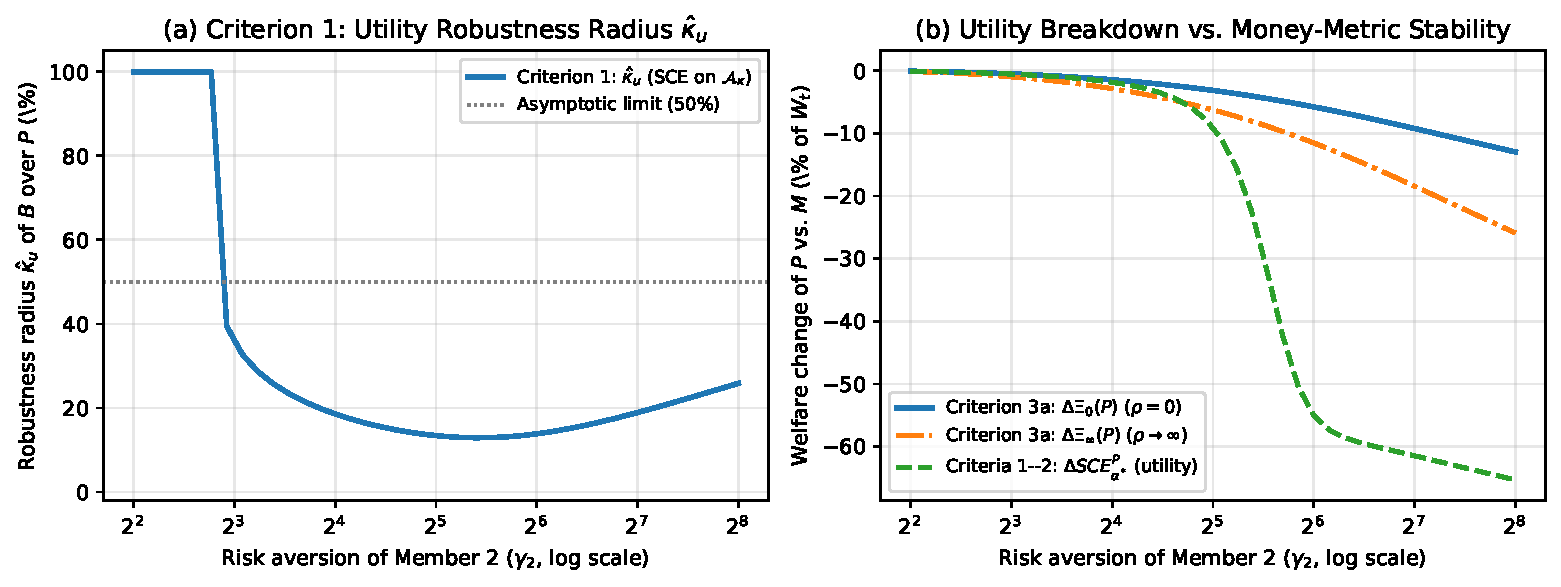
\includegraphics[width=\textwidth]{fig_sec9_gamma_grid.pdf}
  \caption{Sensitivity of Criterion 1 utility robustness radius ($\hat{\kappa}_u$) and Criteria 1, 2, and 3a welfare losses ($\Delta \Xi_0, \Delta \Xi_\infty, \Delta SCE_{\alpha^*}$) to $\gamma_2 \in [4, 256]$ (log scale, $\gamma_1 = 2$, Market A; for $\gamma_2 \le 4.3$, $B$ Pareto-dominates $P$).}
  \label{fig:sec9_gamma_grid}
\end{figure}

\subsubsection*{Part B: Synthesizing Criteria 1, 2, 3a, and 3b in the KT Pool under Transfers and Lotteries.}
To include the ex-post solidarity criterion $SCE_\rho^{\text{ep}}$ (Criterion 3b), which requires a common per-unit utility $v$, we return to the five-member heterogeneous-wealth KT pool of Section \ref{Sect:Het_Participants_Unique_Weights} in Market A ($W_i \in \{0.5, 0.75, 1.0, 1.5, 2.25\}$, $W_t = 6$). Alongside `Prop`, baseline `LEL-CE`, and `LEL-CE rand`, we evaluate a market-inconsistent rule, $\text{LEL-CE}(\tau = 1\%)$, which scales each member's baseline LEL-CE payoff by $(W_{i,t} + T_i)/W_{i,t}$ with $T_5 = -0.01 W_{5,t} = -0.0225$ ($-1.0\%$ of $W_{5,t}$), $T_1 = +0.0225$ ($+4.5\%$ of $W_{1,t}$), and $T_2 = T_3 = T_4 = 0$. Because $\pi_t(W_{i,t+1}^{\text{LEL-CE}}) = W_{i,t}$, this rule transfers exactly $0.0225$ of present market value from Member 5 to Member 1 while leaving Members 2, 3 and 4 unaffected. Under the homothetic reference-point scaling $\text{ref}_i(m_i) = (1+r)m_i$, each participant's equivalent-contribution ratio satisfies $m_i^k / W_{i,t} = CE_{i,t}^k / CE_{i,t}^{\text{AD}} = (CE_{i,t}^k / W_{i,t}) / y^{\text{AD}}$, where $y^{\text{AD}} = CE_{i,t}^{\text{AD}} / W_{i,t} = 1.03503$ is the common Global AD certainty-equivalent return in Market A. Both Criteria 3a and 3b are evaluated on the common grid $\rho \in \{0, 0.5\}$.

\begin{table}[!htbp]
  \centering
  \footnotesize
  \setlength{\tabcolsep}{2.8pt}
  \renewcommand{\arraystretch}{1.12}
  \caption{Part B: Comparison of deterministic, transfer-subsidized, and randomized rules in the Section \ref{Sect:Het_Participants_Unique_Weights} KT pool (Market A, changes relative to baseline LEL-CE in \% of $W_t$; individual columns in \% of $W_{i,t}$).}
  \label{tab:sec9_kt_synthesis}
  \begin{tabular*}{\textwidth}{@{\extracolsep{\fill}} l rr cr rrr rr @{}}
    \toprule
    & \multicolumn{2}{c}{Indiv.\ $\% \Delta CE_i$} 
    & \multicolumn{2}{c}{Criteria 1 \& 2} 
    & \multicolumn{3}{c}{Criterion 3a ($\Delta \Xi_\rho$)} 
    & \multicolumn{2}{c}{Criterion 3b ($\Delta SCE_\rho^{\text{ep}}$)} \\
    \cmidrule(lr){2-3} \cmidrule(lr){4-5} \cmidrule(lr){6-8} \cmidrule(l){9-10}
    Rule & Member 1 & Member 5 & Crit.\ 1 & $\Delta SCE_{\alpha^*}$ & $\rho{=}0$ & $\rho{=}0.5$ & $\rho{\to}\infty$ & $\rho{=}0$ & $\rho{=}0.5$ \\
    \midrule
    Prop                       & $-1.2077$ & $-1.2077$ & Pareto ($-$) & $-2.0166$ & $-1.1668$ & $-1.1668$ & $-1.1668$ & $-1.2077$ & $-1.2077$ \\
    LEL-CE (baseline)          & $\phantom{-}0.0000$  & $\phantom{-}0.0000$  & Base         & $\phantom{-}0.0000$  & $\phantom{-}0.0000$  & $\phantom{-}0.0000$  & $\phantom{-}0.0000$  & $\phantom{-}0.0000$  & $\phantom{-}0.0000$  \\
    LEL-CE ($\tau = 1\%$ sub.) & $\phantom{-}4.8935$  & $-0.7564$ & Trade-off    & $-0.2366$ & $\phantom{-}0.1199$  & $\phantom{-}0.1099$  & $-0.7308$ & $\phantom{-}0.0000$  & $-0.0047$ \\
    LEL-CE rand                & $\phantom{-}0.1682$  & $\phantom{-}0.1682$  & Pareto ($+$) & $\phantom{-}0.1682$  & $\phantom{-}0.1626$  & $\phantom{-}0.1626$  & $\phantom{-}0.1626$  & $\phantom{-}0.0000$  & $-0.2000$ \\
    \bottomrule
  \end{tabular*}
\end{table}

Table \ref{tab:sec9_kt_synthesis} shows how Criteria 3a and 3b jointly capture cross-sectional transfers and intra-state lotteries:
\begin{itemize}
    \item \textbf{Constant proportionality factor $y^{\text{AD}} = 1.03503$:}
    
    For homothetic rules (`Prop` and `LEL-CE rand`), $\Delta \Xi_\rho(k)$ is independent of $\rho$ and equals the time-$(t+1)$ efficiency gain divided by $y^{\text{AD}} = 1.03503$ ($-1.2077\% / 1.03503 = -1.1668\%$ and $+0.1682\% / 1.03503 = +0.1626\%$), converting time-$(t+1)$ certainty equivalents into time-$t$ equivalent contributions;
    \item \textbf{Subsidized LEL-CE ($\tau = 1\%$):} 
    
    Because each member's LEL-CE payoff is scaled by $(W_{i,t} + T_i)/W_{i,t}$, Members 2, 3 and 4 are unaffected ($\Delta CE_2 = \Delta CE_3 = \Delta CE_4 = 0$), while Member 1 gains $+4.8935\%$ and Member 5 loses $-0.7564\%$. As we can see Criterion 2 leads to an overall fund welfare loss of $-0.2366\%$, while for small value of $\rho$ we get a fund gain of about 0.10\%, which reverses for larger values of inequality aversion;
    \item \textbf{Randomized LEL-CE (`LEL-CE rand`):} 
    
    Every ex-ante criterion (Criteria 1, 2, and 3a for all $\rho \ge 0$) ranks `LEL-CE rand` strictly above `LEL-CE`, whereas the ex-post criterion $SCE_\rho^{\text{ep}}$ (Criterion 3b) strips out the lottery gain at $\rho = 0$ ($0.0000\%$) and reverses the ranking to $-0.2000\%$ at $\rho = 0.5$.
\end{itemize}


\section{Comparison with \citet{BalterSchweizer2024}}
The so-far analysis has several similarities with the one of \citet{BalterSchweizer2024}. They can be summarized in the following points:
\begin{enumerate}
    \item Rejecting Utilitarian Utility Sums in Favor of Two-Stage Money-Metric Aggregation
    \begin{itemize}
        \item \citet{BalterSchweizer2024} reject \citet{Harsanyi1955} utilitarian sum of expected utilities because utility scales are unidentified and due to Nozick's "utility monster", where in the absence of risk a utilitarian social planner confuses heterogeneity in risk aversion $\gamma_i$ with heterogeneous tastes for sure wealth, which means that "an agent whose utility for resources is so great that it dominates the planners preferences" \citep{BalterSchweizer2024}. The authors propose a two-stage functional, where first the CE are computed and then aggregated across agents with the inequality-averse outer utility function $v(c) = \frac{c^{1-\eta}-1}{1-\eta}$, where $\eta$ is their inequality aversion parameter;
        \item At the same time, we showcase exactly in Section \ref{Sect:Example} the "utility monster", which appears in utility-based aggregation and very high risk aversion $(\gamma_2 \to \infty)$. In Section \ref{Sect:Money_Metric_Comparison} we adopt exactly this two-stage architecture of Balter \& Schweizer's $\mathcal{E}[v(CE(\gamma, m))]$, with our inequality-aversion parameter $\rho$ corresponding directly to their $\eta$.
    \end{itemize}
    \item Initial Wealth Heterogeneity
    \begin{itemize}
        \item In Remark 11 of \citet{BalterSchweizer2024} note that when initial wealth $V_0(\gamma)$ varies across agents, their unnormalized aggregator $\mathcal{E}[v(V_0(\gamma) CE(\gamma, m))]$ distorts the density of risk types by $V_0(\gamma)^{1-\eta}$ unless $\eta = 1$ (logarithmic social utility), where we follow the notation of the authors;
        \item In our Section \ref{Sect:Money_Metric_Comparison} we resolve this distortion for all values of inequality aversion $\rho \geq 0$ by dividing individual CEs (or equivalent contributions) by initial wealth $W_{i,t}$ inside the power function and weighting by contribution shares $W_{i,t}/W_t$.
    \end{itemize}
    \item The Rawlsian Dictatorship of the most risk-averse agent and the Equivalence between $m_i^k / W_{i,t}$ and the Regret Ratio $CER(\gamma, m)$
    \begin{itemize}
        \item In Lemma 6 of \citet{BalterSchweizer2024}, we get that $CE(\gamma, m) = \exp\big(rT + (\mu-r)mT - \frac{1}{2}\gamma m^2 \sigma^2 T\big)$ is strictly decreasing in $\gamma$ for any risky exposure $m > 0$, the most risk-averse type ($\gamma = b$) always has the lowest raw certainty equivalent. Consequently, both the Rawlsian limit ($\eta \to \infty$) and the Wald maxmin game (Lemma 6) degenerate into a dictatorship of the most risk-averse agent $\gamma = b$;
        \item We also identify this behavior on raw CEs via \citet{FleurbaeyManiquet2011}. Even under the complete-market rule $M$ (where every agent receives their personal Merton optimum $m^*(\gamma_i)$), the more risk-averse agent has a lower raw CE return ($CE_i^M / W_{i,t} = (1+r)\exp(\theta^2 / 2\gamma_i)$), so an inequality-averse planner on raw CEs would transfer wealth from Agent 1 to Agent 2 purely to compensate Agent 2 for being more risk-averse.
        \item To fix this issue \citet{BalterSchweizer2024} propose the Certainty Equivalent Regret Ratio
        \begin{equation*}
            CER(\gamma, m) = \frac{CE(\gamma, m)}{CE(\gamma, m^*(\gamma))}
        \end{equation*}
        where $CE(\gamma, m^*(\gamma))$ is the agent's unconstrained Merton certainty equivalent (again in their notation). We replace the raw $CE_{i,t}^k$ with the Equivalent Contribution at Market Prices $m_i^k = \min\{\pi_t(X) : \E(u_i(X)) \ge \E(u_i(W_i^k))\}$. In the CRRA complete-market lognormal setting of Section \ref{Sect:Example}, an agent with endowment $m_i^k$ investing optimally in the Merton portfolio achieves certainty equivalent $m_i^k (1+r)\exp(\theta^2 / 2\gamma_i) = m_i^k (CE_{i,t}^M / W_{i,t})$. Setting this equal to $CE_{i,t}^k$ yields:
        \begin{equation*}
            \frac{m_i^k}{W_{i,t}} = \frac{CE_{i,t}^k}{CE_{i,t}^M} = CER(\gamma_i, k)
        \end{equation*}
        Hence, our wealth-normalized $m_i^k$ corresponds directly to the Certainty Equivalent Regret Ratio of \citet{BalterSchweizer2024}, provided that we look at the setting of Section \ref{Sect:Example} (where the authors work in a similar setting). While \citet{BalterSchweizer2024} motivate this ratio via \citet{Savage_1972}, we utilize the idea of \citet{FleurbaeyManiquet2011} money-metric utility, which gives us the added power to decompose $m_i^k - W_{i,t} = T_i^k - D_i^k$ into value transfers ($T_i^k$) and deadweight loss ($D_i^k$) for general non-linear risk-sharing rules.
    \end{itemize}
\end{enumerate}
Overall, while there are many similarities to \citet{BalterSchweizer2024} we extend the work of the two authors to a risk-sharing settings, where we look at several possibilities for sharing the risk among the members of the pension scheme. We do not consider ambiguity over the population distribution of risk aversion (like \citet{BalterSchweizer2024}), but try to determine the optimal social planner Pareto weights and look at robustness over the inequality parameter $\rho$. Furthermore, we allow for both CRRA preferences and also non-concave loss aversion utility of \citet{KahnemanTversky1979}. Finally, \citet{BalterSchweizer2024} look at only ex-ante aggregation of certainty equivalents, while we also consider the situation in which we can penalize intra-state lotteries.


\section{Welfare Losses from Parameter Misspecification}
The main idea of this section is to showcase how parameter misspecification influences welfare and to see whether this misspecification leads to more severe welfare losses than imposing the concave envelope. We will look at the case where the planner misspecifies a baseline agent with $\eta_{\text{true}} = 2.25$ \citep{KahnemanTversky1992} and solves the allocation rule under the assumed parameter and not under the true one. The fund will erroneously calibrate the contract using a misspecified $\eta_{\text{assumed}} \in \{1.50, 1.75, 2.00, 2.75, 3.00, 4.00\}$. The exercise is also performed for $a_{\text{true}} = 0.88$ and $a_{\text{assumed}} \in \{0.50, 0.70, 0.80, 0.92, 0.95\}$ and for $b$ with the same values. We do this for all market scenarios and compute the welfare loss in the following manner (for $\theta \in \{\eta, a, b\})$:
\begin{enumerate}
    \item The correctly calibrated benchmark solves the LEL-CE rule using $\theta_{\text{true}}$, yielding terminal wealth $W^*(\theta_{\text{true}})$ with certainty equivalent:
    \begin{equation*}
        \text{CE}^* = u_{\theta_{\text{true}}}^{-1}\left( \E^\P\big( u_{\theta_{\text{true}}}(W^*(\theta_{\text{true}})) \big) \right)
    \end{equation*}
    \item The rule is evaluated under the true parameter $\theta_{\text{true}}$:
    \begin{equation*}
        \text{CE}_{\text{realized}} = u_{\theta_{\text{true}}}^{-1}\left( \E^\P\big( u_{\theta_{\text{true}}}(W^*(\theta_{\text{assumed}})) \big)\right)
    \end{equation*}
    \item The welfare loss in percentage of initial wealth $W_{i,t}$ is:
    \begin{equation*}
        \text{Loss}(\%W_{i,t}) = 100 \times \frac{\text{CE}^* - \text{CE}_{\text{realized}}}{W_{i,t}} \geq 0
    \end{equation*}
\end{enumerate}
The results for this are shown in Table \ref{tab:parameter_misspecification}.
\begin{table}[H]
  \centering
  \small
  \caption{Parameter Misspecification: Certainty Equivalent Loss (\% of $W_i$)}
  \label{tab:parameter_misspecification}
  \vspace{0.4em}
  \begin{tabular*}{\textwidth}{@{\extracolsep{\fill}} l rrrrrr @{}}
    \toprule
    Market Regime & \multicolumn{6}{c}{Assumed Parameter Value} \\
    \midrule
    \multicolumn{7}{@{}l}{\textbf{Panel A: Loss Aversion ($\eta = 2.25$)}} \\
    \addlinespace[0.2em]
    \textit{Assumed $\eta$:} & $1.50$ & $1.75$ & $2.00$ & $2.75$ & $3.00$ & $4.00$ \\
    \addlinespace[0.2em]
    A       & $0.5724$ & $0.2685$ & $0.1164$ & $0.0000$ & $0.0000$ & $0.0121$ \\
    B       & $0.8474$ & $0.5531$ & $0.2497$ & $0.0000$ & $0.0000$ & $0.0000$ \\
    C  & $0.4570$ & $0.1458$ & $0.0458$ & $0.0217$ & $0.0311$ & $0.0492$ \\
    D      & $0.6871$ & $0.3735$ & $0.1351$ & $0.0000$ & $0.0000$ & $0.0000$ \\
    E     & $0.5987$ & $0.3061$ & $0.1268$ & $0.0000$ & $0.0000$ & $0.0000$ \\
    F    & $0.3813$ & $0.0838$ & $0.0139$ & $0.0110$ & $0.0147$ & $0.0220$ \\
    \midrule
    \multicolumn{7}{@{}l}{\textbf{Panel B: Gain Curvature ($a = 0.88$)}} \\
    \addlinespace[0.2em]
    \textit{Assumed $a$:} & $0.50$ & $0.70$ & $0.80$ & $0.92$ & $0.95$ & --- \\
    \addlinespace[0.2em]
    A       & $0.6052$ & $0.3865$ & $0.1749$ & $0.0000$ & $0.0949$ & --- \\
    B       & $0.9100$ & $0.6263$ & $0.2163$ & $0.8012$ & $1.3516$ & --- \\
    C  & $0.7620$ & $0.4448$ & $0.1446$ & $0.0230$ & $0.0455$ & --- \\
    D      & $0.7821$ & $0.5284$ & $0.2978$ & $0.1525$ & $0.6261$ & --- \\
    E     & $0.7098$ & $0.4666$ & $0.2524$ & $0.0000$ & $0.0784$ & --- \\
    F    & $0.7952$ & $0.4389$ & $0.1073$ & $0.0142$ & $0.0225$ & --- \\
    \midrule
    \multicolumn{7}{@{}l}{\textbf{Panel C: Loss Curvature ($b = 0.88$)}} \\
    \addlinespace[0.2em]
    \textit{Assumed $b$:} & $0.50$ & $0.70$ & $0.80$ & $0.92$ & $0.95$ & --- \\
    \addlinespace[0.2em]
    A       & $0.0121$ & $0.0056$ & $0.0019$ & $0.0000$ & $0.0000$ & --- \\
    B       & $0.0198$ & $0.0079$ & $0.0020$ & $0.0000$ & $0.0000$ & --- \\
    C  & $0.0005$ & $0.0000$ & $0.0004$ & $0.0002$ & $0.0004$ & --- \\
    D      & $0.0093$ & $0.0051$ & $0.0016$ & $0.0007$ & $0.0001$ & --- \\
    E     & $0.0068$ & $0.0026$ & $0.0015$ & $0.0000$ & $0.0000$ & --- \\
    F    & $0.0011$ & $0.0006$ & $0.0003$ & $0.0006$ & $0.0009$ & --- \\
    \bottomrule
  \end{tabular*}
\end{table}

% --- Bibliography ---


\bibliographystyle{apalike}
\bibliography{references}
\end{document}
